\chapter{Architecture and Implementation}\label{ch4}

Research on architectures for Web servers have been conducted for years since the Web itself scales rapidly with the ever-growing traffic. One focus in such research is scalability, which can be even defined with more restrictions as, executing concurrent tasks efficiently on modern computing hardwares with multiple cores integrated. Originally handling concurrent requests in Web servers was introduced by the scenario that connections from multiple clients need to be accepted at the same time in order to better utilize the CPU during I/O operations \autocite{kovatsch2015scalable}, which is more a requirement for connection-based protocol like HTTP. Though CoAP takes a different way compared with HTTP, the stage of request processing is similar and concurrency support is still necessary when facing a busy traffic. Different server architecture evolves over a decade, from which M. Lanter \autocite{lanter2013scalability} and M. Kovatsch \autocite{kovatsch2015scalable} have summarized the most significant ones as following, Multi-Process (MP), Multi-Threaded (MT), Single-Process Event-Driven (SPED), Asynchronous Multi-Process Event-Driven (AMPED), Stage Event-Driven Architecture (SEDA) and Multi-Threaded Pipelined (PIPELINED). 

The first attempts of improving server performance was to employ more processes or threads in order to better utilize the CPU(s), which was easy to follow (as one process/thread to one user/request mapping was used and sequential logic could still be applied) but has been proved too expensive in terms of creation time, memory usage and context-switching. The following event-driven style architecture offers better performance especially on single core as it is non-blocking and fewer threads are created and reused during the lifetime of an application. However, both methods have their pitfalls. 

At a logical level, all server-side frameworks and applications have concurrent threads of control that transform the state space in a collaborative fashion \autocite{UCAM-CL-TR-769}. Nevertheless, using threads directly as a programming model adds complexity in both data and control plane \autocite{UCAM-CL-TR-769}\autocite{Lee:2006:PT:1137232.1137289}. Threading model usually assumes a shared memory in which the updatable state resides and different threads of control take turns directly modifying the state space in-place. A variety of locking mechanism are used to guard and serialize the updates to the shared state in order to synchronize among threads. This can make for a highly concurrent system, but is extremely error-prone and hard to reason about especially when it is combined with object-oriented programming, because the later then limits the visibility that certain portions of a program have into portions of the state and effectively partitions the state space \autocite{Lee:2006:PT:1137232.1137289}. Threads are also not a practical abstraction in distributed computing as the effort to make a shared memory illusion is expensive \autocite{Lee:2006:PT:1137232.1137289}. On the other hand, the asynchronous, non-blocking event-driven code essentially consists of a single thread with a main loop which waits and processes events accordingly. Because the thread of control is not interrupted preemptively, which in turn ensures that state updates can be made consistently without using locks, event-driven style often provides simplicity and performance over a multi-threaded architecture \autocite{UCAM-CL-TR-769}. However, event-driven inverts the control flow and effectively turns a program into reactive style, which makes it more complicated to block and harder to understand when the problem space increases \autocite{von2003events}. Also event-drive often assumes a uniprocessor context when compared with multi-threads model, and therefore would underperform under a multi-core or many-core environment. There exist attempts to combine the two paradigms where many single-threaded event-driven processes cooperate together. Such effort, however, still suffers from the synchronization issues mentioned before \autocite{von2003events}.

Concurrency in software is difficult and using threads as a concurrency abstraction makes it worse \autocite{Lee:2006:PT:1137232.1137289}. Non-trivial multi-threaded programs are difficult to comprehend. On the other hand, because threads are insufficient from a footprint and performance perspective, using threads as software unit of concurrency can not match the scale of the domain's unit of concurrency today anymore. As an alternative, programmers have to use constructs that implement concurrency on a finer-grained level than threads and support concurrency by writing asynchronous code that does not block the thread running it, which are, however, hard to write, understand and debug as well \autocite{java-loom}. Moreover, since today's modern hardwares are equipped with multi-core or even many-core chips, which are essentially distributed systems themselves, the assumption of threading model makes it harder to be transparently portable and fully utilize the underlying hardwares \autocite{UCAM-CL-TR-769}. 

With all above being said, as \textcite{Lee:2006:PT:1137232.1137289} pointed out, alternative paradigm such as concurrent coordination languages with actor-oriented style of concurrency should be put more attention to. A language with actor paradigm built-in such as Erlang, though does not fully qualify a proper concurrent coordination language, still compensates many shortages of the threading model. An actor in Erlang is an Erlang process which is lightweight enough and can be started and destroyed very quickly, therefore allowing 
much easier design patterns that could use as many processes as needed. And code can be written in a linear, blocking, imperative style. All above greatly eases the burden of modelling the domain problem. On the other hand, actors have isolated memory and can only communicate using message passing, which avoids the problems and mistakes such as low-level data races and the subtleties of memory models associated with the current shared-memory paradigm \autocite{UCAM-CL-TR-769}. Moreover, as a functional programming language, data is immutable in Erlang and messages between actors are copied in most cases, which further enhances this feature. Compared to languages where data are mutable and can be referenced by pointers, the 
forementioned point could lead to inefficiency, which, however is a trade-off for fault-tolerance.

Erlang has strong fault-tolerance support since its background was rooted in telecommunication industry, which may not be a common feature in other actor based solutions. The first writers of Erlang treat availability and reliability more important than other features in order to develop systems that ``never stop". As a dynamic typed language, Erlang has facilities that help upgrade an online system without any shut down time, which is also known as ``hot code reload". When it comes to faults, instead of preventing errors and problems, Erlang assumes they happen from time to time and provides good way to handle them. It is proved that the main sources of downtime in large-scale software systems are intermittent or transient bugs \autocite{candea2003crash}. And errors which corrupt data should make the faulty part of the system to die as fast as possible in order to avoid propagating errors and bad data to the rest of the system \autocite{learn_you_some_erlang}. So the Erlang way of handling failures is to kill processes as fast as possible to avoid data corruption and transient bugs. The sharing-nothing, immutable data, avoiding locks and other safeguards in Erlang ensures a crash is the same as clean shutdown \autocite{learn_you_some_erlang}. And the ability of an Erlang process to receive signal when other process of interest terminates enables a supervision tree structure in an application, where the leaf nodes being workers who execute actual tasks and parent nodes being supervisors that can take immediate actions upon accidental termination of its children (worker nodes), such as reboot the worker to a known state. Such a structure effectively separates error handling and application logic. The idea is also called ``Let it crash",  which on one hand prevents programmers from over defensive-programming, on the other hand let the application only handle exceptional cases that are expected while hiding unexpected intra-system failures from the end users since they are already as self-contained as possible, improving the perceived reliability of the service. One can still dig into errors and failures afterwards to diagnose though, since this mechanism does not aim at ignoring errors (they are properly recorded anyway) but saves the system from crash upon the very error occurs. The fault-tolerance model of Erlang is not a new one, robust computer systems use similar strategies more or less \autocite{gray1986computers}. However, few environment provides such a finer-grained level of control over faults as Erlang does.

The actor model Erlang based on supports transparent distribution which makes it identical whether two communicating processes locate at the same machine or not. This is achieved by passing messages in a total asynchronous manner so that no assumption of the communication results is made \autocite{learn_you_some_erlang}. The transparent distribution benefits both scaling and fault-tolerance. It naturally transfers to multicore processors in a way that is largely transparent to the programmer, so that one can run Erlang programs on more powerful hardware or over multiple machines without having to largely refactor them. Having concurrent Erlang VMs running and talking through message passing, the same pattern of communicating, detecting failure and relaunching or handling things can be applied on the far end. The asynchronous message passing also makes it possible for user shell or any other code, run as an Erlang process, to inspect the status of a remote virtual machine and manipulate the system with much less effort than other solutions.  

Erlang runs on a virtual machine that has preemptive scheduling and per-process garbage collection built-in, which is vital for the runtime to achieve soft real-time, another telecom industry requirement. Preemptive scheduling is not as efficient as cooperative scheduling which is used in language like Go, but is more consistent, meaning that millions of small operations can't be delayed by a single large operation that doesn't relinquish control. 

The characteristics mentioned before not only render Erlang as a successful telecom industry language, but also make it suitable in Web service where high concurrency and fault-tolerance are needed, such as Web servers and chat service. In this work, it is argued that the Internet of Things share similarities with these areas. With new paradigms such as Fog Computing emerging, IoT intends to be made up of more distributed computing force where latency is sensitive, scaling onto heterogeneous platforms ranging from embedded devices to cloud backends. Erlang should fit well in such circumstances. 

Erlang itself is no silver bullet though. It is particularly inappropriate to use Erlang in signal/imaging processing, number crunching or any other CPU-intensive tasks. And it could be slower than other solutions because the language is dynamic typed and running on a virtual machine. Preemptive scheduling as well as all other effort towards high concurrency and fault-tolerance also brings overhead, which makes Erlang only perform better than other solutions under proper domain problems/workloads, such as busy server-side applications with lots of network traffic but few heavy computing tasks. However, since any non-trivial application is unlikely to be powered by single technology, the patterns used in Erlang are also applicable to other languages. For instance, Akka \autocite{akka} is an open-source toolkit for building concurrent and distributed applications on the JVM, which is written in Scala and emphasizes the actor-oriented programming model over others. A .NET version is also available. Kilim \autocite{srinivasan2008kilim}\autocite{UCAM-CL-TR-769} is a Java actor-oriented server framework which does the magic by transforming the Java bytecode. Project Loom \autocite{java-loom} is a proposal that intends to introduce Fibers (similar concepts to actors) into the JVM. Complex server-side systems usually use a mixture of multiple languages and consist of isolated subsystems that communicate using well-defined messages \autocite{UCAM-CL-TR-769}. This resembles actor-oriented Erlang system anyway. It is the maturity of the language and runtime that renders Erlang as the primary interest of research in this thesis.

\section{Concurrency Model}

The popular Java CoAP framework Californium was inspired by previous work for highly concurrent Internet services, in particular SEDA and the PIPELINED architecture \autocite{lanter2013scalability}. However, much of its assumption is invalid in a concurrency-oriented language context, since creation and synchronization of lightweight processes is much cheaper. Therefore, a more intuitive and straight forward architecture similar to Multi-Process (MP) is still an attractive option. The primary goal of the design is to allow scalability and fault-tolerance following the idiomatic concurrency-oriented language way, that is, isolation of processing, data and faults. 

\begin{figure}[!htbp]
\centering
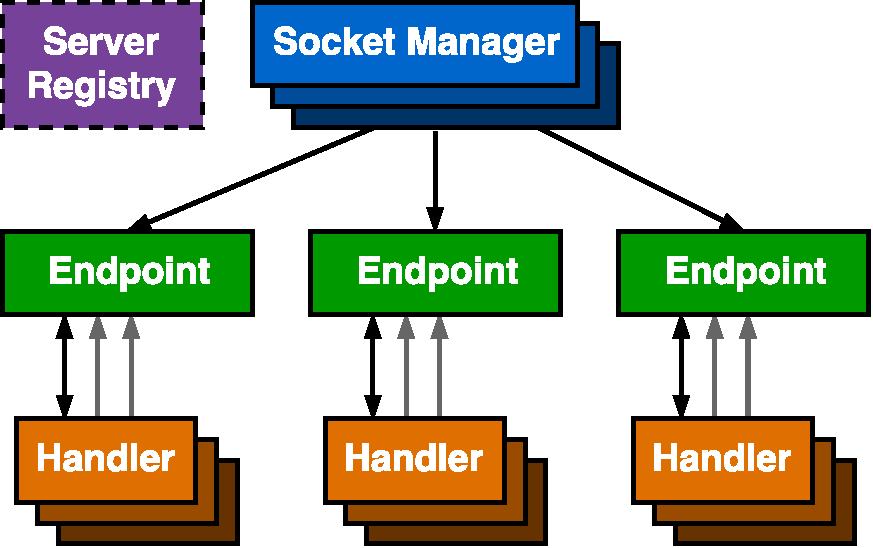
\includegraphics[scale = 0.55]{ecoap_logic_arch}
\caption[The logical architecture of ecoap]{The logical architecture of ecoap. One or more socket manager(s) exist depending on the underlying transport protocol. One endpoint maps to exact one remote CoAP endpoint. Each endpoint may have many handlers associated with it. Handler contains logic for server or client. A server registry is only used for routing in server.}
\label{fig:ecoap_arch_logic}
\end{figure}

It is a common design pattern among Erlang applications to model truly concurrent activity each as a separate process. Therefore it is straight forward to come up with the architecture shown in \autoref{fig:ecoap_arch_logic}. Conceptually, the ecoap prototype can be split up to socket manager, endpoint and handler, which are reusable for both server and client. When being used as server, a registry maintaining routing rules is also included. The socket manager hides network details and would only dispatching received datagrams to endpoints. Thus its number depends on how the underlying transport protocol works. For plain CoAP which is built above connection-less UDP, there is a single instance of the socket manager. While for alternative transport such as DTLS, there might be one socket manager per endpoint. The endpoint represents an actual remote CoAP endpoint, and is created following a one-to-one mapping scheme. It executes the protocol and would let the handler to invoke business logic via a RESTful interface. Depending on the role of the system, different handlers are to be used. It should be noticed that not only the endpoint has a one-to-one mapping against real CoAP endpoint, the handler each maps to an independent CoAP operation as well, where an operation may contain one or more CoAP message exchanges that are logically related. Therefore it is possible to have thousands of endpoint processes each having one or more working handler process(es) all running concurrently and only communicate though message passing, which provides a fine-grained concurrency model that ranges from network level to business logic level. It should be further noted that while the handler executes the business logic, it only requires a pre-defined interface is implemented and has no other limits, which means the business logic can have its own concurrency model as well. The model is much like a pipeline besides all stages of the pipeline are spawned dynamically and have a clear mapping to real world concurrent activities. 
 
On the other hand, these processes will be organized in different ways depending on whether the system runs as server or client, and also some other application-specific requirements, primarily for fault-tolerance considerations. In order to compose a well-defined fault-tolerant application, supervisor processes are necessary to glue the above components together to eventually form a supervision tree. Only by combining the concurrency model with the supervision tree could the proposed prototype achieve essential scalability and reliability. 

With the above in mind, the subsequent sections are organized as follows. Details of each component are discussed respectively from \autoref{socket_manager} to \autoref{coap_registry} while different supervision strategies and the structure of the whole application are introduced in \autoref{supervision_tree}. Then \autoref{state_management} analyzes how states are managed in such a share-nothing environment with special challenges coming with CoAP. 

\subsection{Socket Manger}\label{socket_manager}

The workhorse of the socket manager is an Erlang process which holds the socket. It is responsible for receiving binary data over the network and applying flow control if desired. 
It therefore abstracts the transport protocol, which is UDP in plain CoAP. Though out of scope of this thesis, the component can be easily replaced by wrapping a socket that listens on DTLS port or over other transport layer. The main difference would be instead of a single instance that is known by all endpoints, a connection-oriented alike transport protocol will render more socket processes to match concurrent connections and therefore a one-to-one mapping for socket process and endpoint applies. 

With plain CoAP, the socket manager becomes the only place where data traffic goes through, as the received datagrams are also sent as plain Erlang messages to the process by the runtime. In order to avoid bottleneck, the process should do as little work as possible. When the socket process receives a datagram from a new remote endpoint as server, it starts a local endpoint process and passes the datagram to it together with the source address and port. When a client intends to issue a request towards a server that is not touched before, the socket process starts a local endpoint process as well and passes the provided destination address and port to it so the client can use the component to send the request. The endpoint processes are monitored by the socket manager to maintain a dynamic dispatch table so that it can hands received datagrams to corresponding endpoint process immediately, as shown in \autoref{fig:coap_socket_manager}. The dispatching is based on the inner process dictionary of the socket process. A process dictionary is a destructive local key-value store in an Erlang process. It should be noted that process dictionary destroys referencial transparency and makes debugging difficult \autocite{erl_proc_dict}. It is primarily used to store system information used by the VM that does not change a lot during the lifetime of a process. However, when being used with care (packaging its operation inside well-defined API which does not touch other states), process dictionary provides faster reading/writing performance than other key-value stores in Erlang. Thus the process dictionary is used as a fast dispatch table where the key is a tuple of remote endpoint address and port, and the value is the process identifier (PID) of the worker process that receives messages from the endpoint in the rest time of processing. 

\begin{figure}[!htbp]
\centering
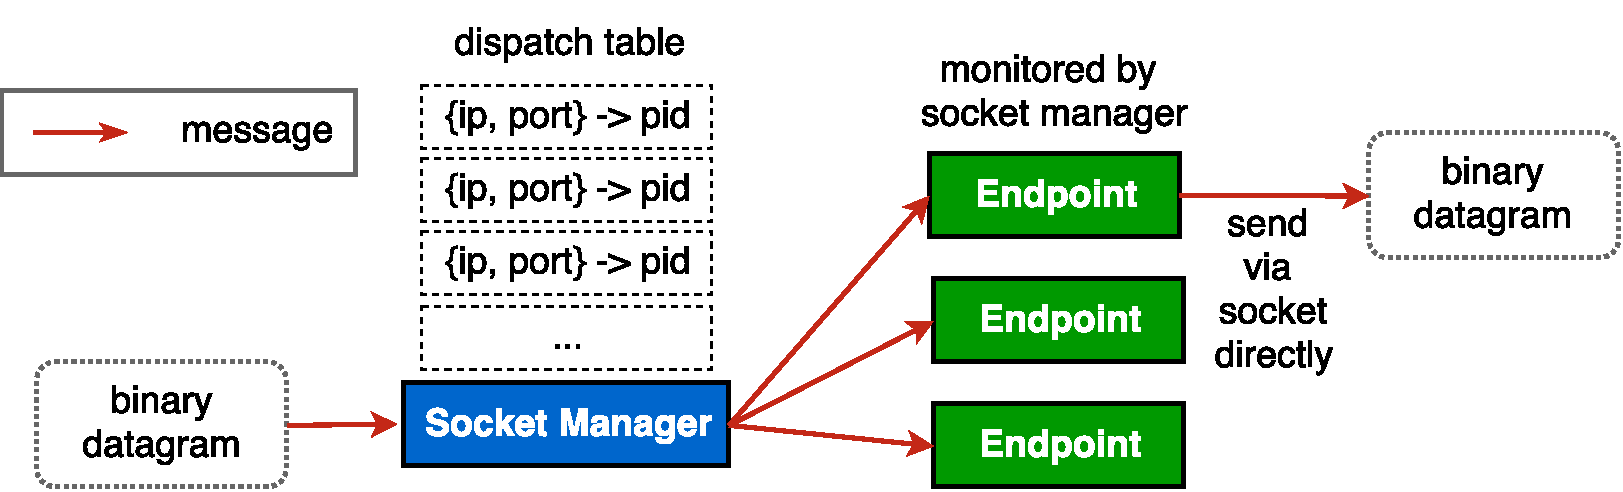
\includegraphics[scale = 0.55]{coap_socket_manager}
\caption[The socket manager]{The socket manager receives datagram over network and dispatches them based on its endpoint dispatch table. The endpoint process sends datagrams directly using the socket reference passed by the socket manager. Every endpoint process is monitored by the socket manager so that the latter would notice its termination.}
\label{fig:coap_socket_manager}
\end{figure}

An interesting feature of the Erlang runtime is while only the owner process of a socket can read data from it, any other process can write to it as long as the process has access to the socket reference. This behaviour can be used to improve port parallelism. So, it is desirable that the socket reference is also passed to the endpoint process when it is created, which enables the worker to send messages directly over the network without further bothering the socket manager. A function that encapsulate sending operation is provided by the socket manager module, which can be invoked by endpoint processes. It is a direct function call without any message passing and hence leaves the socket process alone. This largely reduces the work load of the socket manager process and makes the dispatching between socket manager and endpoint processes a totally asynchronous manner.

Though it is possible to improve data throughput by letting multiple processes listen on the same port, each holding a different socket, this behaviour largely depends in underlying operating system and does not behave well universally. On the other hand, having a single process instead of many simplifies the management of socket and data dispatching.

\subsection{Endpoint}\label{coap_endpoint}

An endpoint process is the representation of the actual remote CoAP endpoint inside ecoap. Because of the low cost of creating and destroying processes in Erlang, a one-to-one mapping is taken here, which means CoAP messages from one remote endpoint are guaranteed to be handled by the same endpoint process during the active session.

\begin{figure}[!htbp]
\centering
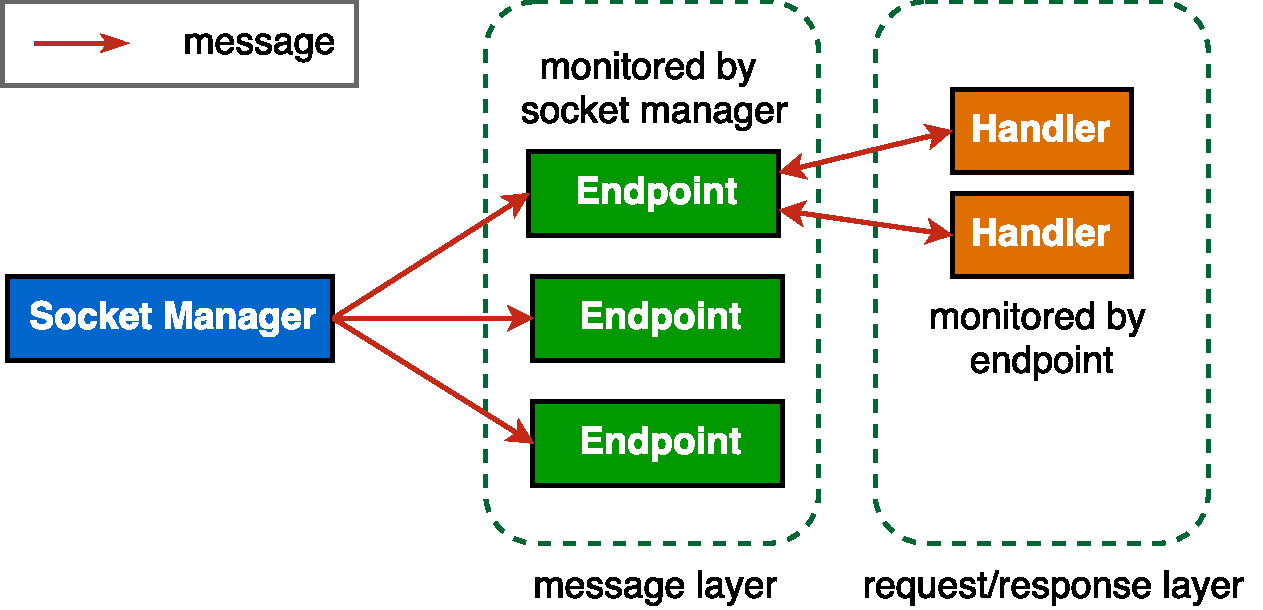
\includegraphics[scale = 0.55]{coap_endpoint}
\caption{Relation between endpoint and handler}
\label{fig:coap_endpoint}
\end{figure}

\begin{figure}[!htbp]
\centering
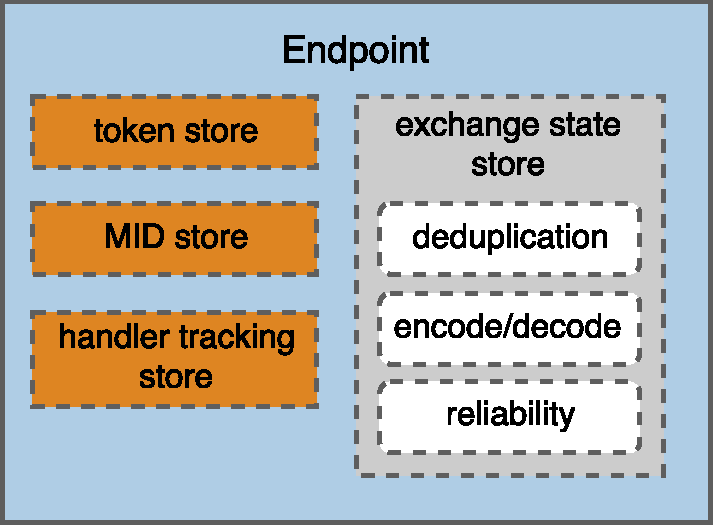
\includegraphics[scale = 0.55]{coap_endpoint_inner}
\caption[The function of an endpoint]{The function of an endpoint. The exchange state is the description of both the current state and the action that should be taken upon the state next. Therefore, deduplication, serialization and reliable transmission are all defined as part of the actions and are executed accordingly.}
\label{fig:coap_endpoint_inner}
\end{figure}

As shown in \autoref{fig:coap_endpoint} and \autoref{fig:coap_endpoint_inner}, the endpoint process wraps the implementation of CoAP message-layer. It is responsible for decoding and encoding CoAP messages, checking duplicates and optional retransmission for reliable message exchange. The process handles above tasks by tracking message exchanges and maintaining a state machine for each of them. An exchange should contain one request and its corresponding response or an empty message while different exchanges may have logical relations, for example, a block-wise transfer or an observe notification renders a request followed by potentially many responses. Using state machine for protocol stage transition is relatively easy and clear and different types of message exchange can have different state machine implementations. However it is unpractical to make every state machine an independent process because the potentially huge amount of message exchanges could lead to too many processes within the system. Instead, the message exchange state contains the description of both the current state and the next action to be taken upon the state. The endpoint process then stores the exchange state as part of its inner state. In such a way, it can process multiple message exchanges asynchronously without spawning new processes. For instance, an incoming confirmable message could render a state as ``finishing message parsing and delivering to handler process but still waiting for corresponding acknowledgement", together with the function name that triggers transition to next state. The very endpoint process can store this exchange state and process other CoAP messages while waiting. When the corresponding acknowledgement arrives as Erlang message, it can fetch the stored exchange state and continue executing it via invoking the state transition function by the fetched function name. The dynamic and functional nature of Erlang enables this feature without much effort. On one hand, the function name is part of the exchange state and can be stored as data. On the other hand, the runtime can use the name to refer to an executable function located in the same file as the exchange state is defined. In similar ways, retransmission can be done by setting timers that will trigger resending if no state transition that cancels them happens before the final time out. Detailed state transition flowchart can be found in \autoref{exchange_implementation}.

The work flow can be briefly described as follows. After receiving the incoming datagram, the endpoint process checks duplication first and triggers corresponding actions upon the exchange state if it is a duplicate. Otherwise, a new state is initiated where the CoAP message is decoded into ecoap's inner presentation and handed to appropriate handler process for further processing. After the handler process finishes its task, it passes the result back to the endpoint process which then  triggers a state transition where actions including encoding the result and sending it over the network are executed.

The endpoint process sets a one-way monitor on every handler process so that it can be notified when they terminate (either a clean finish or a crash). This has an important impact on the lifespan of an endpoint process, which will be discussed later in \autoref{state_management}. 

The endpoint process also manages CoAP message identifiers and tokens when it needs to issue a CoAP message proactively, i.e. being a client or sending a non-confirmable/separate response as a server. The message identifier, or MID, is generated sequentially starting from a random number within the MID range, but independent among different endpoint processes. The share-nothing of Erlang renders MID management straight forward since there is no concern of collision out the scope of a single CoAP endpoint. Within one endpoint one should still make sure that a MID is not reused before corresponding exchange lifetime ends. The message token is generated as a strong random bytes using Erlang's crypto library with configurable length. Tokens are also only produced by endpoint process independently. One could argue that randomly generating token does not fit in a variety of scenarios. However, using crypto strong random bytes as token within one endpoint's scope greatly simplifies the effort for synchronization and avoids collision to a relatively high level, which is enough for the ecoap prototype. While MID is stored as an integer, the endpoint process stores the token in a key-value store which maps request token to the identifier of the request issuer. The token store is necessary for matching incoming responses to requests and dispatching them to corresponding issuers.

\subsection{Handler}\label{coap_handler}

In general, a handler process serves as the request/response layer in CoAP as in \autoref{fig:coap_endpoint}. Depending on the role of the system, the handler process can acts as:

\subsubsection{Server}

An \verb|ecoap_handler| process is used to execute server-side logic, including invoking CoAP resource handler functions, server-side block-wise transfer and observe management, as shown in \autoref{fig:ecoap_handler}. 

\begin{figure}[!htbp]
\centering
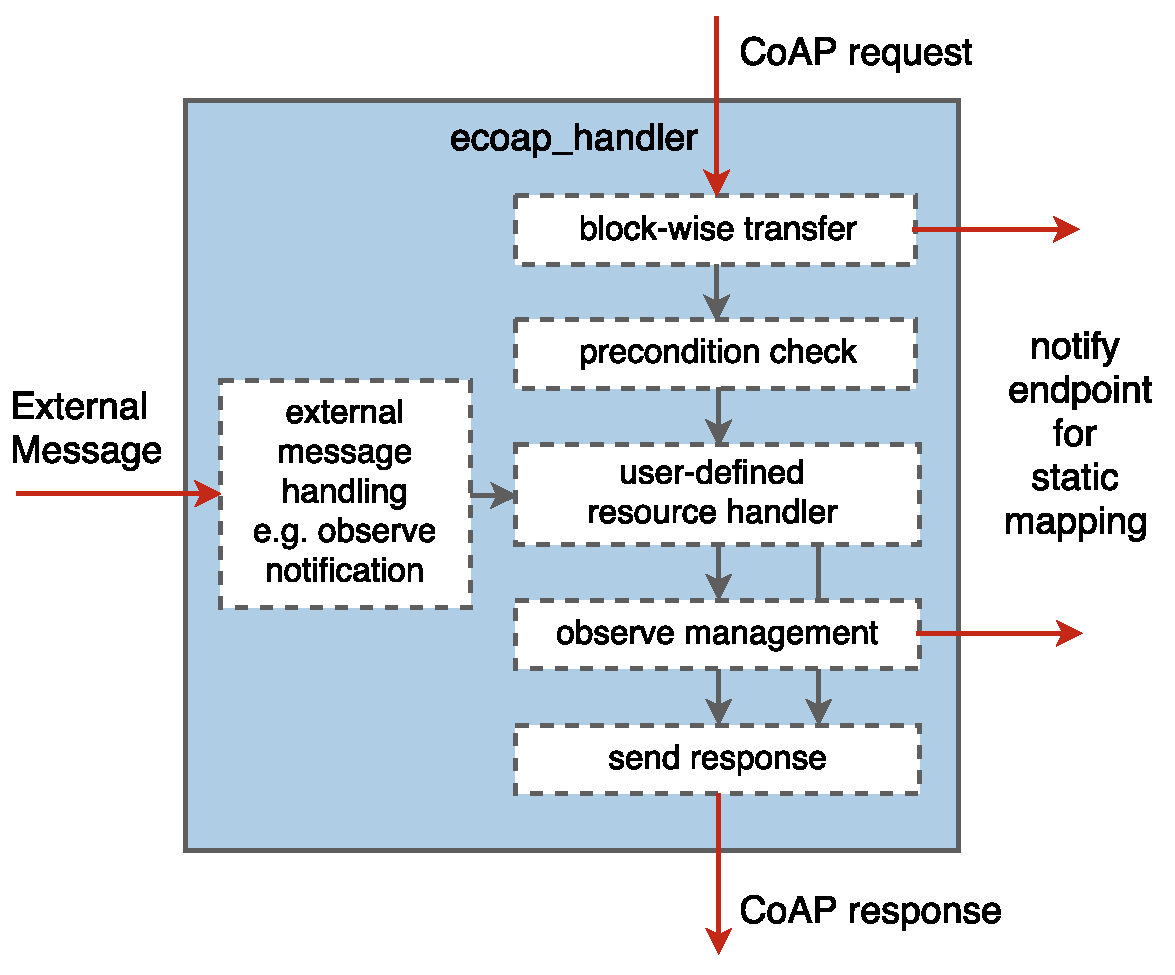
\includegraphics[scale = 0.55]{ecoap_handler}
\caption{Workflow of an ecoap\_handler process}
\label{fig:ecoap_handler}
\end{figure}

A CoAP resource provides a RESTful interface and can be accessed and modified through reacting to requests that carry one of the four request codes defined in CoAP: GET, POST, PUT, or DELETE. One can define a CoAP resource by implementing its handler functions as callbacks required by \verb|ecoap_handler|, which is similar to an interface in object-oriented programming, and register the mapping of resource URI to the module name of the handler functions at the CoAP Registry. When a request arrives at the server, eventually a \verb|ecoap_handler| process searches the registry for a resource that corresponds to the destination URI of the request. If the \verb|ecoap_handler| process finds the resource, the handler functions are executed to process the request and responds with an appropriate response code, options and payload according to the protocol specification, otherwise a 4.04 (Not Found) error code is responded. The assembled response is then passed back to corresponding endpoint process which sends it to the client via the network. 

The \verb|ecoap_handler| process is spawned by the endpoint process on demand and on the fly. For any ordinary request, there is usually one \verb|ecoap_handler| process per request, and the process terminates immediately after sending the response. No  bookkeeping work other than monitoring is taken by the corresponding endpoint process. As a result, requests can be processed concurrently in an intuitive, sequential and blocking fashion. It should ease programming effort especially when the resource handler has to execute certain time-consuming task as it does not need to worry slowing down the server. The Erlang runtime scheduler will make sure all processes share the time slot fairly. If the request has to be responded timely, for instance, a confirmable request, its corresponding message exchange state machine will sets a timer while waiting for the \verb|ecoap_handler| process, so that an empty acknowledgement can be delivered to the client if the handler process fails to finish before time out event. The late result automatically becomes a separate response that is included in a new message exchange. 

However, for block-wise transfer and observe requests, an \verb|ecoap_handler| process keeps serving following requests which query the same resource in the exact same way. In detail, subsequent requests to one particular resource with the same CoAP method and query (CoAP Uri-Query option) as the first request will be processed by the same \verb|ecoap_handler| process as long as there is an ongoing block-wise transfer or observe relation towards that resource. The \verb|ecoap_handler| process lives until the block-wise transfer completes, or the client cancels the observe relation. While requests not subjected to this limitation are handled as normal in newly spawned processes.

This is achieved as follows. After checking the request, the very \verb|ecoap_handler| process informs the corresponding endpoint process its intention to be alive and the latter records its identifier as a combination of CoAP method and query so that subsequent requests matching the identifier can be delivered correctly. Since an endpoint process always monitors the handler process, it will be informed on termination of the handler process and remove the mapping information. This serves two purposes. The first one is it greatly simplifies block-wise transfer and observe management. An \verb|ecoap_handler| process handling a block-wise transfer works in an atomic fashion as defined in RFC7959 \autocite{blockwise}. For a block-wise GET, it caches the complete representation of the resource at once for the client to retrieve step by step, in order to avoid unnecessary resource fetching or possible inconsistence caused by the resource changing frequently. For a block-wise PUT or POST,  it gradually collects the data uploaded by the client and updates the target resource in one action, so that no intermediate state could be seen by others. The static mapping effectively avoids inconsistent resource state being spread over multiple places. On the other hand, when handling observe relation establishment, an \verb|ecoap_handler| process registers itself to \textit{pg2}, a distributed named process groups application that comes with standard Erlang distribution, with the resource URI as the group name. In such a way, \verb|ecoap_handler| processes serving different clients can join one group if the clients intend to observe the same resource. One can then notify the clients recent update of the resource of interest by simply sending the update as Erlang message to the group name, which will be broadcasted to all registered processes by \textit{pg2} afterwards. Eventually each \verb|ecoap_handler| process will assemble an observe notification and push it to the corresponding client. The static mapping again avoids separation of states and provides a clear model. Moreover, the \textit{pg2} application ensures a group is properly cleaned when any of its member process exits. It even works in a distributed environment out of the box, where processes located on different machines can join one group and receive messages, with basic race conditions and partitions handling mechanism \autocite{pg2_failure}, which enables ecoap to scale out with minimum effort. Other process group applications with similar functionality can be placed here as well. The second benefit is that requests that are not related to ongoing block-wise/observe activity can still be handled concurrently just as other ordinary requests, no matter whether they come from the same client or not. Since block-wise transfer and observe are essentially stateful operations, only employing static mapping for them renders each operation as isolated and self-contained as possible while obtaining a balance between high concurrency requirement and maintaining states on server side.

\subsubsection{Client}

The \verb|ecoap_client| process encapsulates request composing, client-side block-wise transfer and observe management. 

Synchronous and Asynchronous requests are both supported and implemented via message passing. Any external Erlang process can act as the caller of an \verb|ecoap_client| process and ask it to perform request on behalf of the process. Synchronous calls block the caller process until a response is delivered. Asynchronous calls return immediately with a reference (a tag that is unique within an Erlang runtime). The response will later be delivered as message to the caller process, which can be pattern matched against the request reference so that the request and response are associated. 

Different from ordinary request calls, synchronous and asynchronous observe calls both have a reference in their return values. The synchronous observe calls also return with the first notification along with the reference. Proactive observe cancellation calls are provided in the same manner as observe calls. When a user process asks the \verb|ecoap_client| process to observe a resource when it is already being observed, the behaviour of \verb|ecoap_client| process is compliant with the re-observe action defined in RFC7641 \autocite{coap_observe}, that is, reusing the same request token.

The \verb|ecoap_client| process also handles block-wise transfer in an atomic fashion, where the response is handed to user process only after the whole exchange completes. Concurrent block-wise transfer is an undefined behaviour \autocite{blockwise}. The \verb|ecoap_client| process deals with this by abandoning the ongoing block-wise exchange and continuing with the newly established one, which is essentially an overwrite and a desired result in many cases.

Moreover, one can use the reference obtained from an asynchronous call to cancel the issued request before the corresponding response is received. If the reference is from an observe call, the observe relation is cancelled in a reactive way, where the next notification from the server will be rejected by sending a reset message. Any ongoing block-wise transfer corresponding to the request is stopped immediately after invoking request cancel call. This is done by turning ongoing block-wise message exchange to a cancelled state where further events such as message retransmission are just ignored.

Multiple user processes can share one \verb|ecoap_client| process since each request/response/observe/block-wise transfer tracking is self-contained and will not interrupt with each other. All tracking data are stored in a key-value store as part of the process inner state, providing fast reads and writes. 

\begin{figure}[!htbp]
\centering
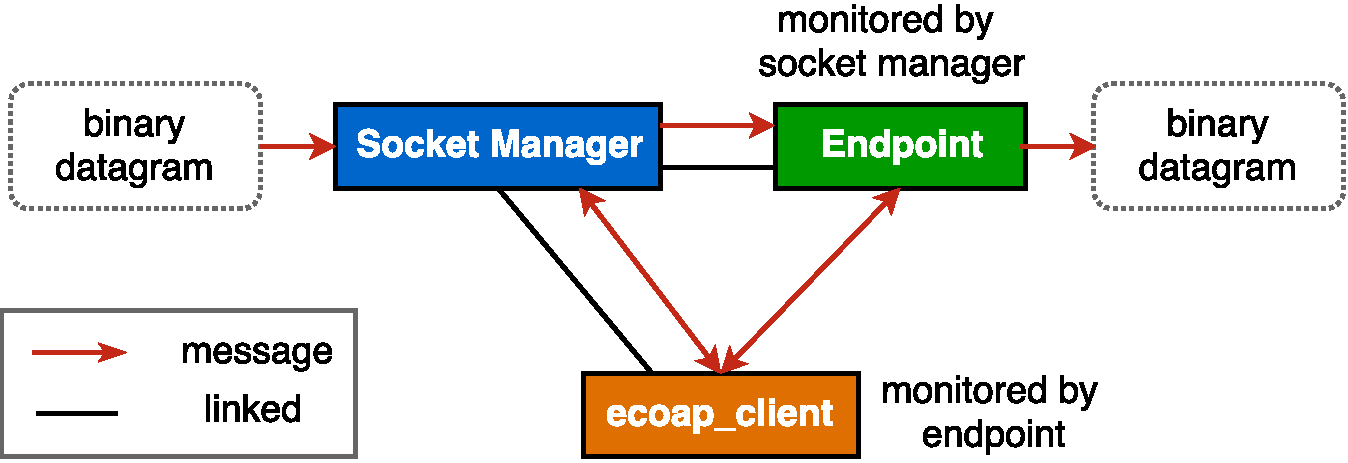
\includegraphics[scale = 0.7]{ecoap_client_standalone}
\caption[Structure of a standalone client]{Structure of a standalone client. The ecoap\_client process only uses message passing to ask the socket manager to start corresponding endpoint process.}
\label{fig:ecoap_client_standalone}
\end{figure}

A client can be started as a standalone one or an embedded one. As a standalone client, the \verb|ecoap_client| process starts a socket manager and links to it. For the socket process, when the \verb|ecoap_client| process issues a request, it directly starts an endpint process and links to it as well (if there is not an existing one), instead of using any other supervision tree structure, as shown in \autoref{fig:ecoap_client_standalone}. Therefore a standalone client consists of one \verb|ecoap_client| process, one socket manager and zero or one endpoint process. The client as a whole can be connected to any supervision tree as usual in a standard way so that one can compose a customized application. The link among processes is to ensure crash of any of them will definitely bring down others and thus avoid orphan process and inconsistent state. 

\begin{figure}[!htbp]
\centering
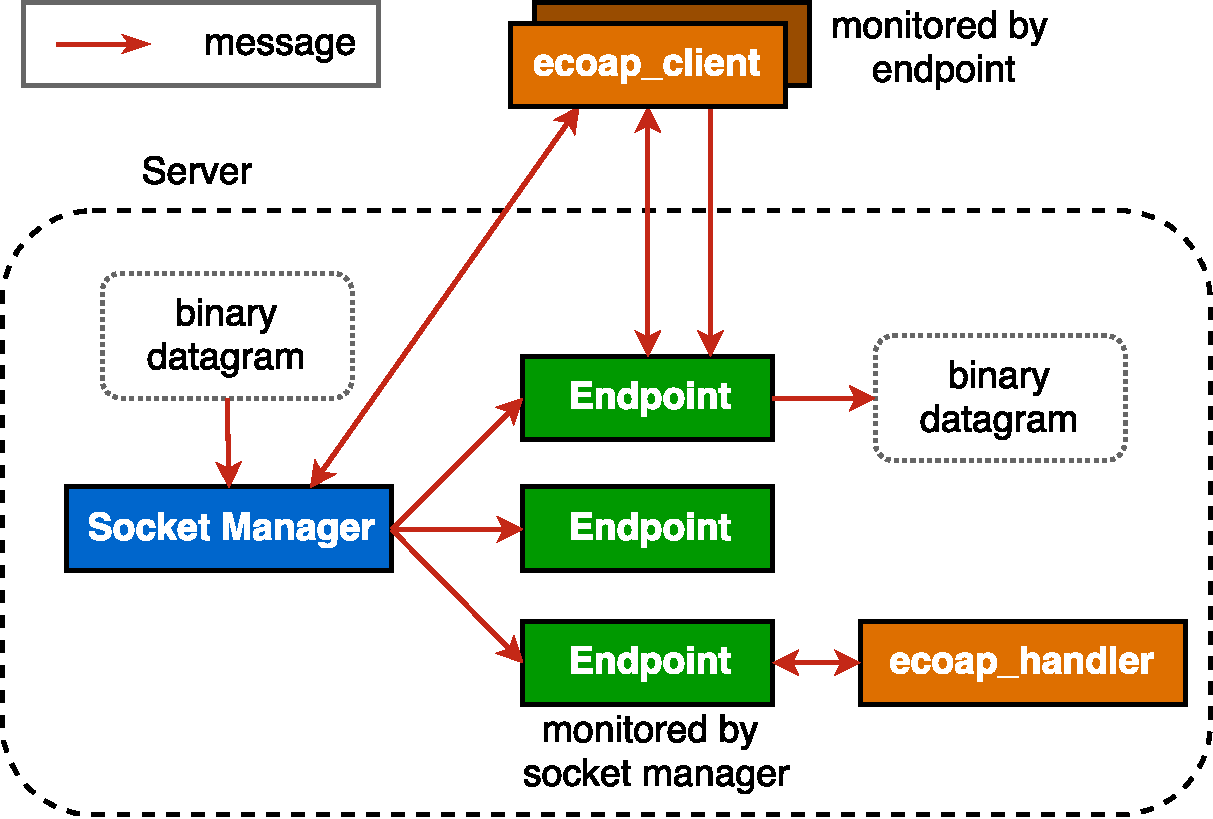
\includegraphics[scale = 0.7]{ecoap_client_embedded}
\caption[Structure of an embedded client]{Structure of an embedded client. The ecoap\_client process is not directly involved in the server but asks the server to send request on behalf of it, so that client and server can share the same network interface.}
\label{fig:ecoap_client_embedded}
\end{figure}

While an embedded client uses existing socket manager instead of spawning one. This can be useful when an application wants to behave as server and client at the same time while sharing the single network interface, like the behaviour defined in OMA Lightweight M2M (LWM2M) \autocite{lwm2m}, an IoT device management protocol built atop CoAP. For instance, an \verb|ecoap_client| process can be started and specified to use the same socket manager of a running ecoap server. Then when issuing a request, the newly created endpoint process will be connected to the supervision tree of the server, and will be used for both client role and server role which avoids duplication and confusion of states within the application. Also, depending on the requirement of the application, the \verb|ecoap_client| process could be started either during the initialization of the server or inside a resource handler function.

The endpoint process monitors the \verb|ecoap_client| process for a special purpose. Assume in the embedded mode an \verb|ecoap_client| process exits due to any reason, the endpoint has to cancel all ongoing message exchanges that the client originated. The endpoint uses the monitor to track this extra information. It is inappropriate to let the endpoint process terminate with the client process as what would happen in a standalone client, because the endpoint process might be used by the server concurrently. In the standalone mode, termination of an \verb|ecoap_client| process will shutdown the socket manager and all alive endpoint processes anyway, no matter the termination is normal or a crash. The monitor is more for a consistent reason other than the purpose stated above. On the other hand, since socket manager is not started by the client process in the embedded mode, there is no direct link between them. Therefore the \verb|ecoap_client| process should monitor the socket manager instead in case it terminates unexpectedly.

The \verb|ecoap_handler| and \verb|ecoap_client| process both work as the handlers that provide interface to business logic. They can both be considered as request/response layer of CoAP. The main difference is they are connected in different ways to the corresponding CoAP endpoint component and supervision strategy varies. This is because server and client have reversed data flow, where the \verb|ecoap_handler| process is the end of request processing in a server while the \verb|ecoap_client| process is the one that begins a request.

\subsection{Server Registry}\label{coap_registry}

A server registry is essentially a manager for routing rules of a server. For the sake of simplicity, a key-value based routing is used in the ecoap prototype, where the key is the URI of resource presented as a list of path strings and the value is corresponding resource handler module name. 

The routing rules are stored in an Erlang Term Storage (ETS), which is an efficient in-memory database built in Erlang VM that allows limited concurrent operations. In most cases a data structure is hold by an Erlang process as its internal state and the process acts upon it through message passing with other processes. However when the data structure needs to be shared with many processes, this isolation makes the single process a bottleneck. The ETS provides a way to store large amount of data with constant access time. It also allows concurrent destructive operations with some restrictions (See \autocite{ets} for more details). It acts like a separate process with its own memory but can be configured to allow direct accessing from other processes. In the case of this thesis, reading the routing rules occurs at most of time instead of writing, which renders ETS a fast and reasonable solution. 

\begin{figure}[!htbp]
\centering
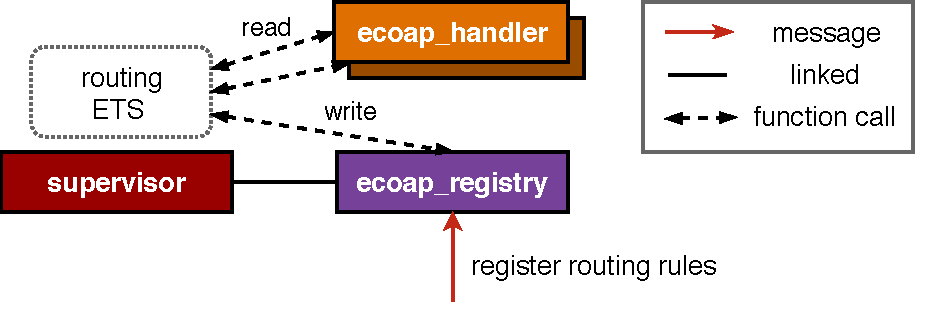
\includegraphics[scale = 0.7]{coap_registry}
\caption[Supervision tree of the server registry]{Supervision tree of the server registry. The routing ETS table is owned by the supervisor. The ecoap\_registry process serialize all writes to the table including insert and delete. Many ecoap\_handler processes can read from the table concurrently. Reads and writes are direct function call without accumulated messages in a single process.}
\label{fig:coap_registry}
\end{figure}
 
A ETS table can not be linked to or monitored as normal process, but has the concept of ownership. The process that creates the table becomes the owner and the table will be removed after the process terminated or crashed. The table can be configured to allow only the owner to operate (private), only the owner to write and other processes to read (protected) which is the deafult, or any process to read and write (public). In order to improve fault-tolerance, ecoap takes a workaround: let the ETS for routing rules be created by a supervisor process with public access control, but only allow one child process to perform actual write operations. This turns the child process, the \verb|ecoap_registry| as shown in \autoref{fig:coap_registry}, to a table manager which serializes all writes but still gives the permission of reading to all other processes. The structure is based on the assumption that updates to routings seldom happen and will not become a bottleneck. Since the supervisor process does not take part in any other work than monitoring its children, it is unlikely to crash. When the \verb|ecoap_registry| crashes due to any reason, it will be restarted by the supervisor while the table keeps alive. Therefore, instead of one process, the server registry consists of two including a supervisor. 

The matching is done by first searching a key that equals to the resolved URI, and then finding the one with the longest prefix if the former step failed. This way one can have a handler for \verb|/foo| and another for \verb|/foo/bar|. One can also specify whether wildcard in URI is allowed or not. If wildcard is used and a resource handler with the longest matching prefix is selected, the suffix of the resolved URI can be retrieved by the handler function for pattern matching. The matching is exported as a function executed in the context of \verb|ecoap_handler| processes that directly operate on the ETS. 

\subsection{Supervision Tree}\label{supervision_tree}

%Rewrite supervision tree part, with background first

%1. Introduce basic supervision strategy and their usage
%2. Introduce onion theory (error kernel)
%3. With that being said, have the following sup tree
%4. And then explain one part after another...
%5. NOTE: I have revised the supervision tree! Check git log! 

%The philosophy isn't defensive programming, but to design your code to just assume failure and keep going.  These concepts are then extended in the OTP library that comes with the language that extends this philosophy to common service patterns, so the user doesn't even have to roll their own.  Everything about the BEAM and language are designed with the OTP in mind which makes it very effective.

Fault-tolerance is the most important feature of Erlang apart from concurrency. The previous section analyzed the fault-tolerance of the server registry. In this section fault-tolerance policy of other components and the architecture of the whole prototype is presented.

Though true fault-tolerance could not be achieved without distribution and redundancy, the fine-grained fault-tolerance settings in Erlang ensure that a transient error could not bring down an application easily even when it runs on a single node. Fault-tolerance is primarily reached by supervision trees where each supervisor has a separate restarting policy towards their children. 

Erlang follows the convention of an onion-layered approach and tries to identify the \textit{error kernel} of an application. The \textit{error kernel} is where the logic should fail as less as possible or even is not allowed to fail. In order to protect the most important data, as a general rule, all related operations should be part of the same supervision trees, and the unrelated ones should be kept in different trees. While within the same tree, operations that are more failure-prone can be placed deeper in the tree, and the processes that cannot afford to crash are closer to the root of the tree \autocite{learn_you_some_erlang}. This approach decreases the risk of core processes dying until the system can not cope with the errors properly anymore.

Before diving into details, some basic terminologies are given first. First of all, supervisor processes are the ones whose sole work is to make sure their children, the processes spawned by them, are under control when they terminate. By saying under control it means the very supervisor can take proper action upon the termination event, like restart the child process. Worker processes are the ones in charge of doing actual work, and may crash while doing so. Supervisors can supervise workers and other supervisors but workers can only be positioned under one supervisor. They can then form a supervision tree.

There are basically two reasons why a proper Erlang program should always use a supervision tree if it is to spawn any process. The first one is only with supervision tree can all processes belong to one application be tracked. This is important since otherwise one may silently leak process and eventually use up all available memory. The second reason is that supervision tree makes sure an application can shutdown in a determined order. It is simply done by asking the top supervisor of an application to terminate, which will then asks all its children to shutdown. If any of the children is also supervisor, it does the same to its own children until all the tree terminates. In case of unexpected conditions such as a process can not terminate correctly, its supervisor has the option to directly kill the process.

Though there are many considerations when designing a supervision tree, the primary concerns here are the supervisor restart strategy and the child restart type. The supervisor restart strategy defines how a supervisor reacts upon children termination in general, considering the relation between children processes. It can be one of the following:

\begin{itemize}

\item \verb|one_for_one|, which means if a supervisor has many children and one of them terminates, only restart that one. It is usually used when processes are independent from each other.

\item \verb|one_for_all|, which means if a child process terminates, all other child processes are terminated, and then all child processes, including the terminated one, are restarted. This is used when processes under a tree depend on each other to work properly.

\item \verb|rest_for_one|, which means if a child process terminates, all child processes that are started after the one should be terminated as well and all of the child processes are restarted. It is a special case where processes have partial dependencies and start order matters.

\item \verb|simple_one_for_one|, which is a simplified \verb|one_for_one| strategy, where all child processes are dynamically added instances of the same process. While supervisor with other strategy can start its child processes accordingly during the initialization of the supervisor itself, a \verb|simple_one_for_one| supervisor has no child at start and will only add child when being asked for. One of the big difference between this one and \verb|one_for_one| is that \verb|simple_one_for_one| is much more efficient when one has only one type of child process but needs to frequently starts and shuts down any number of them.

\end{itemize}

The child restart type on the other hand specifies what the supervisor should to when that particular child terminates. It can take one of the three values:

\begin{itemize}

\item \verb|permanent|
\item \verb|temporary|
\item \verb|transient|

\end{itemize}

A permanent child is always restarted no matter what (be it a crash or a normal termination). It is often used for vital, long-living process of an application. A temporary child is never restarted no matter what (even if a \verb|one_for_all| is used and a sibling death brings down the temporary process). It is for short-lived worker process that are expected to fail and few other code depends on them. While a transient child is restarted only when it terminates abnormally. It is used when a worker process needs to succeed its job but will not be used later. An application can mix the child restart type with supervisor restart strategy as needed but one has to be aware of the final effect. 

One can also tell a supervisor the restart limits of its children. That is to say, the supervisor will give up and exit if more than maximum allowed restarts happen within specified period of time (in seconds). This exit includes terminating all other child processes that may still be running. And eventually this exit will be handled by the supervisor's supervisor (if there is any).

Other factors that can be taken by supervisors are not discussed here for simplicity and one may refer them to \autocite{otp_supervisor}.

With the forementioned guide in mind, the supervision tree of ecoap is shown in \autoref{fig:system_arch}. This is primarily a supervision tree of a CoAP server since clients structure depends heavily on use cases. 

\begin{figure}[!htbp]
\centering
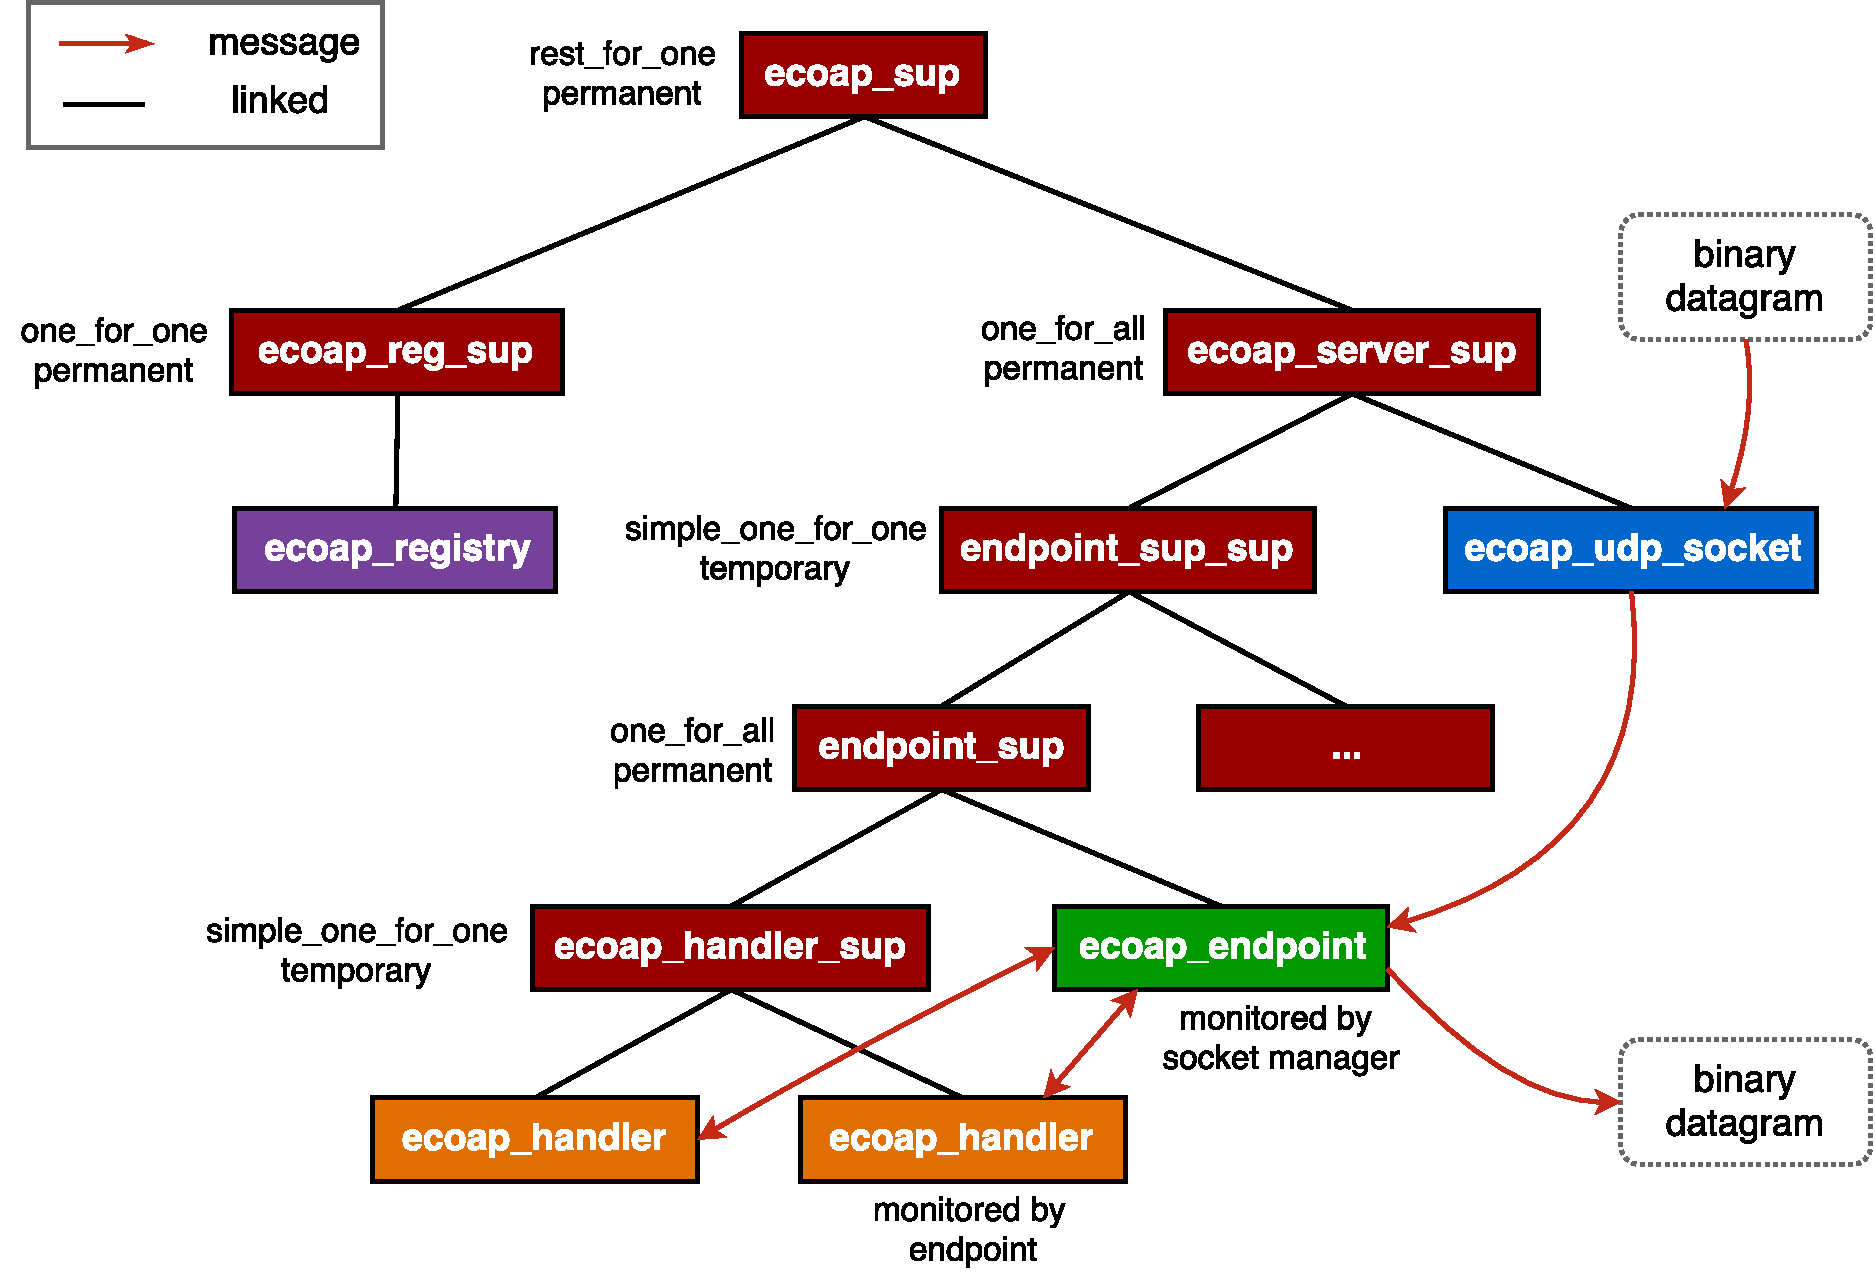
\includegraphics[scale = 0.7]{system_arch_vertical}
\caption{Supervision tree of ecoap as server}
\label{fig:system_arch}
\end{figure}

The \verb|ecoap_handler| process is the deepest node in the whole supervisor tree as it executes user-defined resource handler functions which is a more risky operation. Its supervisor should make no assumption about it and ignores its crash since wether the process succeeded in sending the result is unknown. Instead, the CoAP protocol ensures retransmission of the message so that another \verb|ecoap_handler| process is likely to be started later. 

The characteristics of \verb|ecoap_handler| are obvious: There is no dependency among multiple \verb|ecoap_handler| processes; All \verb|ecoap_handler| processes are dynamically added during runtime; No other type of child process under the same supervisor exists. Based on above observation, a \verb|simple_one_for_one|, \verb|temporary| strategy is the most proper one for the \verb|ecoap_handler| process. With this restart strategy, crash of any \verb|ecoap_handler| process will not cause any restart and will not affect other running processes under the same supervisor.

An \verb|ecoap_endpoint| process is logically connected to corresponding \verb|ecoap_handler| processes since they all represent operations of an active remote CoAP endpoint. Therefore the \verb|ecoap_handler_sup| process should be the sibling of the endpoint process and both under the same tree. The \verb|ecoap_endpoint| process knows this supervisor and asks it to start handler processes.

The \verb|ecoap_endpoint| process is the core of modelling a remote CoAP endpoint. Crash of it usually means all ongoing message exchanges towards the very endpoint becomes invalid. All processes related to the endpoint process should be terminated and the higher level supervisor is not supposed to restart them, since all necessary data for that remote endpoint to continue have lost already. It is also impractical to have failover at this level because it adds obvious synchronization overhead. Instead, ecoap expects the remote endpoint to restart message exchange or retransmit the last message if it is still active and expects further actions. In such a case, a new endpoint process is spawned and everything goes on like normal except the loss of message exchange history, which can render re-execution of certain logic if the duplicate of a message that is received previous to the crash arrives. This can, however, be avoided by well-defined RESTful interface which utilizes idempotent operations or by extra application-layer measures to protect important states. The above actions are needed anyway to implement a reliable service.

It requires the termination of an \verb|ecoap_endpoint| process brings down its supervisor sibling and their common supervisor. While a supervisor process can not be shutdown easily without explicit command, a workaround as follows is taken. The top supervisor, namely \verb|endpoint_sup|, sets \verb|ecoap_endpoint| and \verb|ecoap_handler_sup| both as \verb|permanent| and uses a \verb|one_for_all| restart strategy. Meanwhile the restart limit is set to 0 time in 1 second. This way termination of any of the two child processes would trigger their common supervisor to restart them all but immediately reaches the restart limitation and directly terminate its rest child as well as itself. 

If the tree of \verb|endpoint_sup|, \verb|ecoap_endpoint| and \verb|ecoap_handler| is considered as a compact component, there needs to be another supervisor on top of it so that the socket manager can start new endpoint process via it. This supervisor, \verb|endpoint_sup_sup| should therefore take a \verb|simple_one_for_one|, \verb|temporary| strategy because its situation is similar to \verb|ecoap_handler_sup|. 

Although the single \verb|ecoap_endpoint| process approach is not fault-tolerant enough for a particular remote endpoint, it effectively ensures that faults are isolated between different remote endpoints, improving fault-tolerance performance of the whole system. 

It is worth noting that, when an embedded client reuses the server socket process, any new created \verb|ecoap_endpoint| process still has the \verb|ecoap_handler_sup| sibling, though it may not be put into use. 

The socket process, \verb|ecoap_udp_socket| in the case of this thesis, is the \textit{error kernel} of ecoap. Crash of the socket process implies the socket is closed and any reference to it becomes invalid. In such a case, all endpoint processes can not send CoAP message using the closed socket anymore and must terminate as well. It is possible to make the socket process a named process and let endpoint processes send messages to the socket process which then doing the network sending on behalf of them. Then the crash of socket process does not affect endpoint processes since they only send messages to a named process who will be restarted soon and no other process will compete to register the name. However, this method introduces extra load to the socket process as it effectively serialize the outgoing CoAP messages. More importantly, the socket process maintains its dispatching table inside its process dictionary which is destroyed as soon as the process terminates. Thus the above method turns the system into a situation where only endpoint processes could send messages out but the restarted socket process can not identify them and ignore their existence, rendering an inconsistent state. It is only doable when the dispatching table is outside the socket process, such as in an ETS. Nonetheless, this approach adds risk of race condition and is not considered. 

As a result of that, the supervisor of \verb|ecoap_udp_socket| and \verb|endpoint_sup_sup|, namely \verb|ecoap_server_sup|, takes a \verb|one_for_all|, \verb|permanent| strategy so that when any of these two crashes, they are both restarted immediately. This also ensures that any sub tree under this layer are terminated as well during this restart. For instance, when the \verb|ecoap_udp_socket| process crashes, \verb|endpoint_sup_sup| is also terminated by their supervisor and both are restarted, which also brings down any child under \verb|endpoint_sup_sup|, which then brings down their children accordingly, until all nodes under \verb|endpoint_sup_sup| are terminated (Note the processes marked as \verb|temporary| will not be restarted). After the restart, no orphan endpoint process or blind socket process will exist. The same logic applies to any combination of crashes of the two processes. 

If one considers the above structure with another level of abstraction, the server can actually listen on different ports simultaneously by starting multiple instances of the \verb|ecoap_server_sup| supervisor with different parameters (e.g. the port number), which then starts their own \verb|ecoap_udp_socket| and \verb|endpoint_sup_sup| processes, ready for incoming requests respectively. This way requests towards different ports are also isolated and executed concurrently with minimal effort. And because of reusing existing components, all fault-tolerant features discussed above still apply.

On the other hand, in order to reduce complexity, the server registry does not need an extra supervisor. Instead the routing table is kept by the root supervisor with the \verb|ecoap_registry| process being a direct child of it. Since the registry worker process is independent from the rest of the application, the root supervisor can simply have the \verb|ecoap_server_sup| supervisor as its another child and uses a \verb|one_for_one|, \verb|permanent| strategy. One can then start as many server instances as needed while sharing a single registry process. The root supervisor is then linked to the application controller of the Erlang VM. Crash of the root supervisor implies failure of the whole application thus no further action is taken other than completely shutdown ecoap. This also agrees with the design of the server registry, as the routing table will only be destroyed when the root supervisor is down, in which case there is no point to continue service without human intervention.

%On the other hand, within the server registry, the supervisor sets a \verb|one_for_one|, \verb|permanent| strategy since the \verb|ecoap_registry| process is its only child and should always be restarted after a crash. 

%As shown in \autoref{fig:system_arch}, the supervision tree completes when the \verb|ecoap_server_sup| process and the \verb|ecoap_reg_sup| process both connect to the root supervisor of the application. The root supervisor is then linked to the application controller of the Erlang VM. Crash of the root supervisor implies failure of the whole application thus no further action is taken other than completely shutdown ecoap. It is desired that crash happens to \verb|ecoap_server_sup| should bring down the tree under it but leave \verb|ecoap_reg_sup| alone. While the crash of the \verb|ecoap_reg_sup| process should terminate both of them because the routing table has gone with the \verb|ecoap_reg_sup| process and all subsequent requests will result in a 4.04 (Not Found) response. There is no point to continue service unless one manually initialize the routing table again. For this reason, the start order of \verb|ecoap_server_sup| and \verb|ecoap_reg_sup| is important. If the supervisor starts \verb|ecoap_reg_sup| first and then \verb|ecoap_reg_sup|, and applies a \verb|rest_for_one|, \verb|permanent| strategy to them, it is guaranteed that crash of the later started one will not affect the first started one, but crash of the first started one will bring down both of them. 

In summary, influence of a crash is limited as much as possible to avoid cascade failure and improves the availability of the entire server. Faults happened in one handler process will not affect another handler process, even when they are serving the same client. Similarly, failure of one endpoint process will not be noticed by other remote endpoints. The server will only be considered unrecoverable when the faults causing too many restarts that exceeds the preconfigured maximum restart limit on each layer of the supervision tree until eventually propagating to the top supervisor, which then terminates the whole application. Despite monitoring and restarting failed child processes, the supervision tree also clarifies the dependency of worker processes, making it easier to understand and extend the application.

\subsection{State Management}\label{state_management}

\subsubsection{Deduplication States and Lifespan of Endpoint}

A CoAP endpoint might receive the same message multiple times. Two messages are equal, if their sources, destinations, and MIDs are the same within the same lifetime \autocite{lanter2013scalability}. It is required that a CoAP endpoint remembers confirmable messages for a EXCHANGE LIFETIME (247 seconds) and non-confirmable messages for an NON LIFETIME (147 seconds) \autocite{coap_protocol}. When a duplicate message arrives the server should respond with the same response without re-executing the request (at-most-once semantics). Thus a CoAP endpoint have to cache the response for transmission, along with the request information for filtering. The potential large amount of ongoing requests and the memory they cost require the server to reduce the exchange states and drop them after finishing the requests as soon as possible. 

It is decided that each \verb|ecoap_endpoint| process should maintain a key-value store that maps MID to exchange state instead of using a central bookkeeping. It avoids centralized bottleneck and improves fault-tolerance since the message exchanges in different endpoints are effectively isolated. Each \verb|ecoap_endpoint| process periodically iterates through all entries of the exchange store and checks their age. Any message whose lifetime has expired is removed from the store. It is proved that the above method is more efficient than creating a timer for every message. As timer is also implemented as process in Erlang, using more timers than required would slow down the performance of the endpoint process handling normal CoAP messages. It can be argued that the periodical scan would block the endpoint process. However, the fine-grained concurrency model where one endpoint process maps to exact one remote CoAP endpoint makes it unlikely to accumulate too many entries within one process, rendering the scan blocking an acceptable trade-off in terms of performance. After all, a remote endpoint sending with high frequency could easily reuse MID too early which breaks the protocol anyway. Moreover, this design eliminates any need for synchronization or locking.

It should be noticed that CoAP server can further relax deduplication \autocite{coap_protocol}. First of all, NON requests are less critical as their lifetime is shorter and the semantics indicate their unreliability: they can be designed so that no response needs to be cached and only duplicate filtering is needed. Furthermore, when processing only idempotent requests such as GET, PUT, and DELETE, no responses have to be cached and ecoap can be configured to completely disable deduplication. For computation intensive resources, results can be cached locally. On the other hand, POST requests can be optimized using application knowledge to implement a more efficient deduplication strategy. 

It is also important to determine when a remote endpoint is not active anymore, so that the corresponding \verb|ecoap_endpoint| process can be safely shut down (with the sub supervision tree it links to) and resource being hold can be released. A remote endpoint is considered inactive when all of the past message exchanges have expired, no outgoing request is left uncompleted, and no \verb|ecoap_handler| process is running. All the conditions have to be met at the same time because there are situations where ongoing exchanges exist but the exchange store is empty. For example, when a client is observing a resource that is seldom updated, or waiting for a separate response of a time-consuming task, there is a chance that no new message ever arrives during the wait and all exchanges have expired and been removed. Apparently the endpoint process should not terminate in such a case, be it either on client side or on server side. 

On the one hand, in order to track outgoing requests, the endpoint process simply reuses its token store. Since the token store is cleaned up whenever a request is completed, checking whether it is empty is enough to make sure no request is left open. On the other hand, the endpoint process monitors all alive \verb|ecoap_handler| processes and maintains a counter which tracks the number of them. As a result, it could then directly check whether the corresponding stores are all empty as well as the counter is set back to zero right after each exchange store cleanup to determine if it should terminate or not. However, it is not enough to examine only the above conditions when no deduplication is enabled or when message lifetime is configured to be strongly reduced. The endpoint process might falsely consider it is about to terminate while there is still ongoing traffic on the way because the exchange store is emptied too fast. To avoid this situation, the process should also track whether any message has ever arrived between each cleanup, which can be easily implemented as a flag that keeps being set each time a message is received. To sum up, an endpoint process could only safely terminate after a cleanup on its exchange store when the following items are all true,

\begin{itemize}

\item The last message exchange has expired.
\item The handler process counter is zero.
\item No outgoing request is left uncompleted.
\item No message has arrived between two cleanups. 

\end{itemize}

The four conditions are not valid in all cases, for example, the handler process counter is always zero for a client. But any violation of them implies the remote endpoint may further communicate with the application and corresponding processes should be ready for that. When an endpoint process does terminate, the socket manager will be notified on this event and remove its record from the dispatching table. The sub supervision tree where the endpoint process resides is automatically shut down as described in \autoref{supervision_tree}. 

\subsubsection{Observe States}

The basic observe workflow is introduced in \autoref{coap_handler}. Another challenge is the management of observe notification sequence. Since UDP datagrams can get reordered, observe notifications must carry a strictly increasing sequence number in the Observe option. The client can eventually have the latest representation of a resource by selecting the notification with a higher sequence number and drop the old ones. Generating observe sequence number in a multi-threaded environment with shared memory is complex due to race conditions \autocite{kovatsch2015scalable}. In ecoap, however, the problem is avoided by generating the sequence number within the \verb|ecoap_handler| process. Observe notifications can only be sent by first going through the single \verb|ecoap_handler| process that maintaining the observe relation for the very client, which effectively serializes the notifications in the exact order as they reach the message queue of the process. There is no chance that a first produced notification gets a higher sequence number than the actually latest one does. This method compliances with RFC 7641 \autocite{coap_observe}, which says ``The sequence number selected for a notification MUST be greater than that of any preceding notification sent to the same client with the same token for the same resource." On the client side, things are similar no matter if multiple notifications arrive at the same time or not, as they are received and queued in the single \verb|ecoap_client| process. Regardless of the arrival order, there will not be concurrent processing against the notifications and the single client process can reorder them safely. Because of the fine-grained concurrency model, serialization of the above procedures derives a low cost but simple solution. 

%most software errors are transient errors - crash only software

%preemptive scheduling is not as efficient as cooperative scheduling but is more consistent, meaning that millions of small operations can't be delayed by a single large operation that doesn't relinquish control.

%Let it crash does not imply let it burn

%scalability - it would be much easier to design programs that could have as many processes as needed instead of using process pools.

%shared nothing and reliability - sharing memory could leave things in inconsistent state. etc. 

%fault-tolerance

%1. find good ways to handle errors and problems, rather than trying to prevent them all.
%2. multiple processes with message passing - make error handling a separate logic - clear and easy
%3. share nothing - errors that corrupt data should cause the faulty part of the system to die as fast as possible in order to avoid propagating errors and bad data to the rest of the system.
%4. share nothing - all crashes are same as clean shutdowns
%5. transparent distribution benefits both scaling and fault-tolerance
%6. asynchronous message passing does not make any assumption on receiving side, which allows safe remote function calls

%concurrency impl

%os is not reliable and efficient enough

%The solution is simply to have your program running on more than one computer at once?something that?s necessary for scaling anyway. This is another advantage of independent processes with no communication channel outside message passing. You can have them working the same way whether they?re local or on a different computer, making fault tolerance through distribution nearly transparent to the programmer.

\section{Implementation}

Previous sections explain the architecture of ecoap and how the different parts work together to fulfill the processing chain of CoAP messages. In the following section, a more detailed introduction to how a CoAP message is modelled and how these components can be implemented is given.

\subsection{Process Overview}

Erlang provides the Open Telecom Platform (OTP) framework, which generalizes common design patterns into a set of libraries and export them through Erlang behaviours. Behaviours are formalizations of these common patterns which divide the code of a process into a generic part (a behaviour module) and a specific part (a callback module). The OTP offers a bunch of basic behaviours such as supervisors, finite state machines, event managers and generic servers. One can then use the behaviour by implementing a customized callback module which exports a set of pre-defined callback functions, much like an interface implementation in a OOP context. The OTP and behaviours reduce the complexity in terms of code, testing, maintenance and understanding. ecoap is built all based on standard OTP behaviours. Besides all supervisor processes, which are obviously implementations of the \verb|supervisor| behaviour, the socket manager, endpoint and handler are all using the generic server, namely \verb|gen_server| behaviour. While these components might be more efficient if written without using behaviours, it is considered the increased efficiency does not compensate the lost generality in this work. On the other hand, following the spirit of OTP, ecoap provides its own behaviour as well. One can implement customized resource handler logic by implementing the \verb|ecoap_handler| behaviour, where callback functions for REST verbs and CoAP observe are defined in a consistent manner, as shown in \autoref{api_example}.

The socket manager, endpoint and handler processes communicate mostly in an asynchronous manner using one way \verb|gen_server| cast or direct message passing in order to avoid unnecessary blocking. For example, when the socket manager delivers a CoAP message to corresponding endpoint process, it does not care about the result of this operation and a blocking \verb|gen_server| call serves no purpose here. In case of a process crash, the delivery can safely fail because related processes will be terminated or restarted anyway. The above also applies to the communication between the endpoint process and the \verb|ecoap_handler| process. The only exceptions are with \verb|ecoap_client| process and the server registry, as the former has to provide meaningful results to the client while the latter must ensure an operation such as registering a routing entry be a deterministic and atomic operation to avoid race conditions. Their exposed APIs are therefore \verb|gen_server| calls under the hood, which will bring down the caller if a failure happens, a usual behaviour in many Erlang applications. All communication details are hidden by wrapping the casts/message passing in proper APIs though, so that further changes that are internal to the process can be made smoothly. 

\autoref{fig:ecoap_process_tree} shows the supervision tree of a running ecoap example server through \textit{Observer} \autocite{erlang_observer}, the graphical tool of Erlang which displays system and process information. The example consists of three active clients where one of the clients has established an observe relation towards certain resource hosted by the server. 

\begin{figure}[!htbp]
\centering
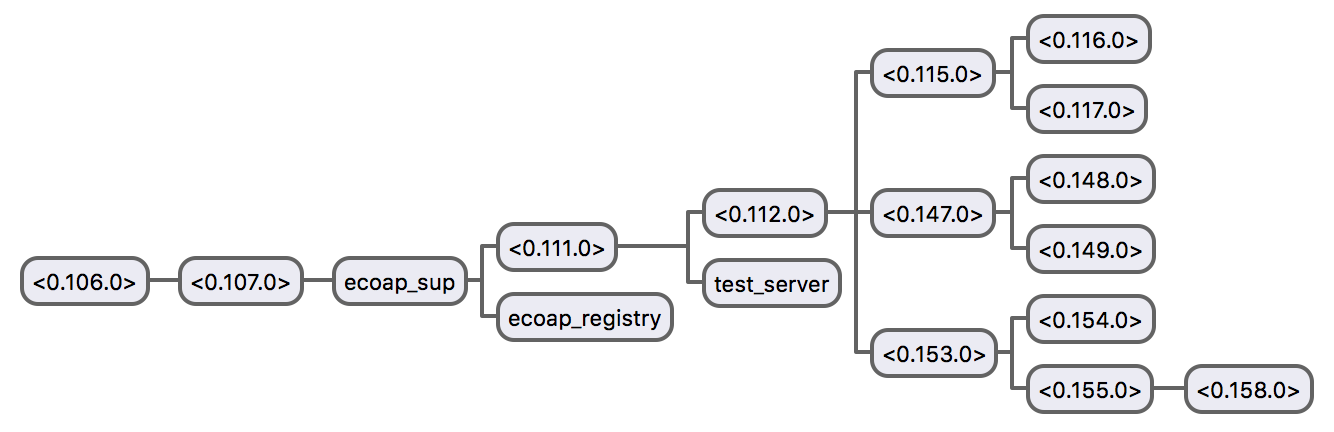
\includegraphics[scale = 0.6]{ecoap_process_tree}
\caption[Process tree of an example server]{The figure shows the process tree of an example server. The 
\textit{test\_server} is an instance of the socket manager process. Process \textit{<0.116.0>},  \textit{<0.148.0>} and \textit{<0.154.0>} are endpoint processes representing three active clients. Among them the client for process \textit{<0.154.0>} has established an observe relation, which is handled by the handler process \textit{<0.158.0>}.}
\label{fig:ecoap_process_tree}
\end{figure}

\subsection{Message}

It turns out simple to implement binary based protocols such as CoAP with pattern matching in Erlang. The following example shows how one could extract different parts of a binary CoAP message with one line of code, where the binary is split to segments separated by comma, pattern matched respectively and bound to corresponding variables. \verb|?VERSION| refers to a pre-defined macro that equals to the current CoAP version and can be seen as a constant. Therefore, \verb|?VERSION:2| matches the first two bits of the binary against the constant so that any binary starts with different two bits fails the match and will not be recognized as a proper CoAP message. After than, fields begin with capital letter are free variables to be bound and the digit follows each field implies the length of the segment to be matched against. For example, \verb|Type:2| binds the second segment (which is two-bits long) to variable \verb|Type| and \verb|Token:TKL/bytes| means binding variable \verb|Token| to \verb|TKL| bytes start right after the 16 bits message identifier (\verb|TKL| is bound earlier in the match and is an integer).  Assume \verb|BinMessage| is a datagram received from network, the binary pattern matching avoids unnecessary parsing effort while legal parts of a message can be obtained effectively without further twiddling with bits. 

\begin{listing}[!htbp]
\centering
\begin{minted}
[bgcolor=bg,
framesep=2mm,
baselinestretch=1.2,
fontsize=\footnotesize
]{erlang}
<<?VERSION:2, Type:2, TKL:4, Class:3, DetailedCode:5, MsgId:16, Token:TKL/bytes, Tail/bytes>> = BinMessage.
\end{minted}
\caption{Example of parsing binary CoAP message through pattern matching}
\end{listing}

It is error-prone and obscure to use the above format all over the application despite the convenient binary syntax of Erlang. Therefore, a CoAP message is further decoded and represented as an Erlang record, which is a syntax sugar of tuple where attributes can be directly accessed by name. \autoref{lst:coap_message_record} and 
\autoref{lst:coap_message_record_example} show the definition of the record for a CoAP message and an example, respectively. Default values can be set within the definition as well as the type of each field. One can then get attributes by only pattern matching against desired ones. For instance, pattern \verb|#coap_message{type=Type, id=MsgId, token=Token}| extracts \mintinline{erlang}|type|, \mintinline{erlang}|id| and \mintinline{erlang}|token| of a message while other parts are ignored. Updating of a record can be done in a similar way. 

\begin{listing}[!htbp]
\centering
\begin{minted}
[bgcolor=bg,
framesep=2mm,
baselinestretch=1.2,
fontsize=\footnotesize
]{erlang}
-record(coap_message, {
    type = undefined :: coap_message:coap_type(),
    code = undefined :: undefined | coap_message:coap_code(),  
    id = undefined :: coap_message:msg_id(), 
    token = <<>> :: binary(),
    options = #{} :: coap_message:optionset(),
    payload = <<>> :: binary()
}).
\end{minted}
\caption[Definition of the CoAP message record]{Definition of the CoAP message record with default values and type information. It is defined as \textit{attribute = default value :: type} where \textit{type} can be native Erlang type such as \textit{binary} or user-defined type expressed as \textit{Module:Type()}. For example, attribute \textbf{token} and \textbf{payload} has a default value of empty binary while attribute \textbf{options} is of map type under the hood.}
\label{lst:coap_message_record}
\end{listing}

\begin{listing}[!htbp]
\centering
\begin{minted}
[bgcolor=bg,
framesep=2mm,
baselinestretch=1.2,
fontsize=\footnotesize
]{erlang}
#coap_message{
    type = 'CON',
    code = 'GET',
    id = 8243,
    token = <<155,209>>,
    options = #{'Uri-Path' => [<<"example">>, <<"one">>]},
    payload = <<>>
}
\end{minted}
\caption[Example of a CoAP message as a record]{Example of a CoAP message as a record. The message is a confirmable GET request for the resource located at ``/example/one" with a MID of 8243 and a two bytes token of [0x9b, 0xd1] (Note each byte is represented as decimal in the figure).}
\label{lst:coap_message_record_example}
\end{listing}

It should be noticed though that record syntax is only valid within the module it is defined. In order to access the definition globally, it must be put in a header file (like a C header file) that is explicitly included by other modules. It is argued that exposing a record across multiple places is not a recommended approach in Erlang applications. However, encapsulating it all by accessor functions reduces a lot convenience on direct pattern matching. Therefore ecoap makes the definition a project-wide header file meanwhile providing functions to manipulate the record, so that one still can obtain attributes without knowing the innards of it. It is a trade-off between expressing ability and maintainability. 

\subsection{Exchange}\label{exchange_implementation}

Instead of using the OTP \verb|gen_statem| behaviour which defines finite state machine to be run as independent process, the state transition of the message exchange is implemented using plain Erlang functions. Similar to message, a record is used to hold useful information of an exchange, including the timestamp and lifetime of the message that initiates it, the current stage of the state machine, cached result for deduplication, timer for triggering any time out event and finally the retransmission counter. The exchange state machine is then completed by combining the exchange record and state transition functions that accept the record as input and manipulate the state according to the information stored in the record.

The endpoint process uses the built-in \verb|map| data structure to store the exchange records. In order to distinguish the incoming and outgoing messages, the exchange records are not indexed by just the MID, but a combination of the direction of message and its MID, like \verb|{in, MID}| or \verb|{out, MID}|. When an endpoint process receives an incoming CoAP message delivered by the socket manager, or an outgoing CoAP message sent by the handler process, or a time out message caused by a timer, it searches the map and invoke corresponding state transition function as specified by the stage stored in the exchange record. The full state transition flowchart is shown in \autoref{fig:exchange_state_transition}.

\begin{figure}[!htbp]
\centering
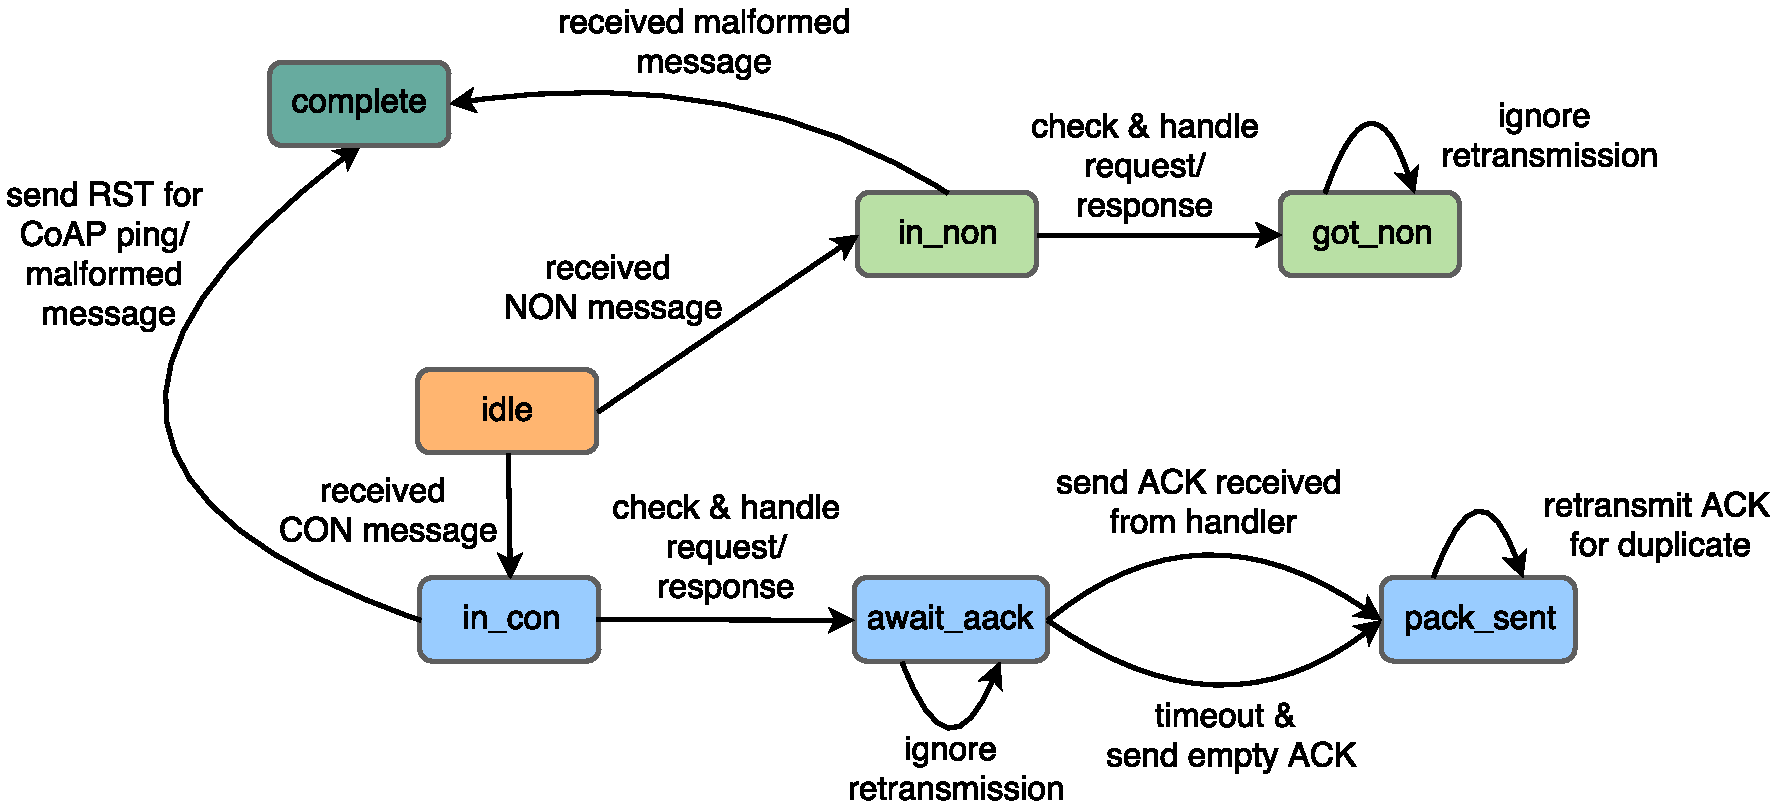
\includegraphics[scale = 0.55]{exchange_state_in}
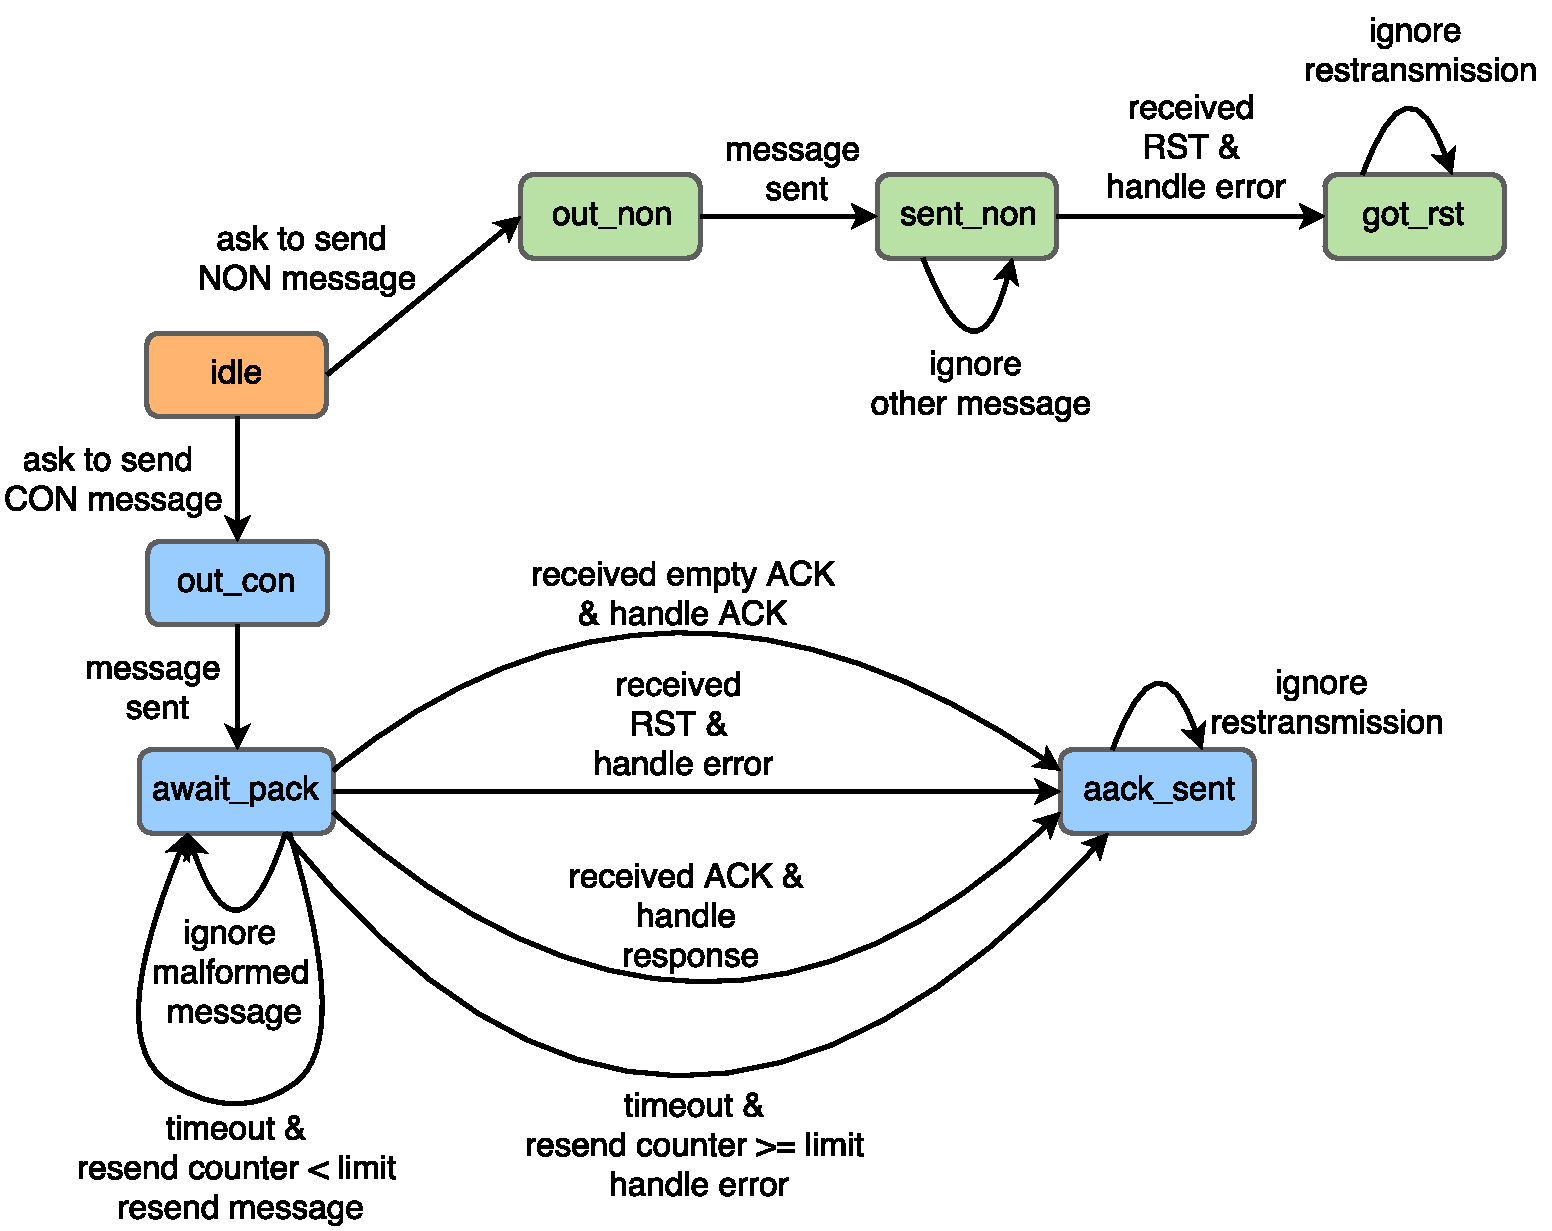
\includegraphics[scale = 0.55]{exchange_state_out}
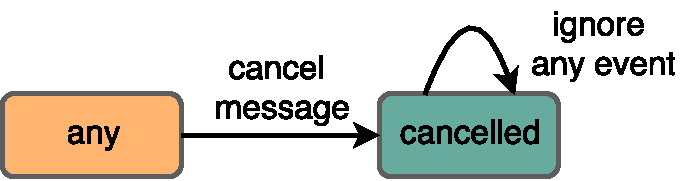
\includegraphics[scale = 0.55]{exchange_state_cancel}
\caption[Exchange state diagram]{Exchange state diagram. All exchange starts from idle state. The complete state means the exchange is immediately removed.}
\label{fig:exchange_state_transition}
\end{figure}

\subsection{API Example}\label{api_example}

The following example shows how a simple CoAP server instance can be constructed with the ecoap prototype. One needs to implement resource handle functions as well as callbacks for observe push events. This is done by implementing the \verb|ecoap_handler| behaviour along with application-specific code. The resource handler needs to be added to the server before it serves any request.  

\begin{listing}[!htbp]
\centering
\begin{minted}
[bgcolor=bg,
frame=lines,
framesep=2mm,
baselinestretch=1.2,
fontsize=\footnotesize,
linenos=true]
{erlang}
-module(example_server).
-export([coap_discover/1, coap_get/4, coap_put/4, coap_delete/4, 
    coap_observe/4, coap_unobserve/1, handle_info/3]).
-export([start/0, stop/0]).
-behaviour(ecoap_handler).

start() ->
    % start ecoap and any application it depends on
    {ok, _} = application:ensure_all_started(ecoap),
    % maps path /HelloWorld to the resource handler that implements ecoap_handler behaviour
    Routes = [{[<<"HelloWorld">>], ?MODULE}],  % ?MODULE refers to current module      
    % server is started with registered name hello_server
    ecoap:start_udp(hello_server, [{port, 5683}], #{routes => Routes}).

stop() ->
    application:stop(ecoap).

% resource operations

% function that returns the description of the resource, if any
coap_discover(Prefix) ->
    % the resource name is the same as its registered path with no extra description
    [{absolute, Prefix, []}].  
    
coap_get(_EpID, _Pefix, _Suffix, _Request) ->
    % reply with 2.05 payload (text/plain) 
    {ok, coap_content:new(<<"HelloWorld">>, #{'Content-Format' => <<"text/plain">>})}.   
     
coap_put(_EpID, Prefix, Suffix, Request) -> 
    Content = coap_content:get_content(Request),
    ecoap_handler:notify(Prefix++Suffix, Content),  % notify all observers
    ok.
    
coap_delete(_EpID, Prefix, Suffix, _Request) ->
    ecoap_handler:notify(Prefix++Suffix, {error, 'NotFound'}),
    ok.
  
coap_observe(_EpID, _Prefix, _Suffix, _Request) ->
    % do something
    {ok, dummy_state}. % {ok, SomeState} where SomeState could be anything

coap_unobserve(dummy_state) ->
    % do something
    ok.

% ObsReq is the origin request that starts the observe, State is the one returned by coap_observe/4
handle_info({coap_notify, Msg}, _ObsReq, State) ->  % observe notifications from ecoap_handler:notify/2
    {notify, Msg, State};  % directly send notification without modification
handle_info(_Info, _ObsReq, State) ->
    {noreply, State}.      % ignore other messages send to the very ecoap_handler process
\end{minted}
\caption{ecoap server API}
\label{lst:ecoap_server_api}
\end{listing}

Resource handle functions has the remote endpoint address, prefix and suffix of request URI and the request itself as parameters. The prefix is the path that represents the resource registered with the server registry while the suffix is any other segments following the prefix (if wildcard is allowed, otherwise empty). One can pattern match against the prefix and suffix to get dynamic URIs, for example, to extract the value of a wildcard or switch to alternative function clause if handlers of multiple routes are implemented in the same module. The \verb|Request| is a CoAP message record underneath and can be used to obtain options and payload via helper functions. The \verb|coap_discover/1| function is used to get the description of a resource as defined in Core Link Format. The \verb|coap_observe/4| function is invoked when an observe relation is established with the resource and would return any useful state valid during the observe. The \verb|coap_unobserve/1| is the opposite of the \verb|coap_observe/4| and should do clean work if needed. The \verb|handle_info/3| function is triggered when the \verb|ecoap_handler| process representing the ongoing observe relation receives resource update message as a result of \verb|ecoap_handler:notify/2| function call or any other message being sent to the process. One can manipulate the notification message in this function or directly forward it. It is also possible to generate an unique reference here if the notification is to be sent as a confirmable message. Then when the message is successfully acknowledged, \verb|coap_ack/2| will be invoked with the very reference to verify this delivery. If no reference is explicitly specified, a dummy value is used. 

In the example, the server is started with registered name \textit{hello\_server} which can be later used to locate the socket process. It can be stopped by calling the \verb|stop/0| function. It has one entry in the routing table which routes requests to \verb|/HelloWorld| to the handler functions implemented in the same module. The GET handle function responds with the text "HelloWorld". The PUT handle function invokes \verb|ecoap_handler:notify/2| to send a new notification with the same content (payload and options) as in the request to all registered observers. The DELETE handle function sends a 4.04 (Not found) response to all observing clients. One may notice that the \verb|coap_post/4| and \verb|coap_ack/2| is not implemented. This is because ecoap sets all the callback functions as optional and a default implementation will be invoked if the user does not provide one. This minimizes redundant code template.

For clients, the \verb|ecoap_client| module exports necessary functions to access a remote server. The module can be used in a similar way as OTP \verb|gen_server|. One needs to call \verb|ecoap_client:open/{1,2,3}| to spawn and links to a \verb|ecoap_client| process and \verb|ecoap_client:close/1| to stop it. The first argument of the \verb|open| function is the hostname or address of the server in the form of \verb|coap://example.me:5683| or \verb|coap://192.168.0.12:5683|, where the port number can be omitted (the default port will be used).
The other optional arguments are the local port to be bound or the socket process to be associated with as an embedded client, as well as other environment settings such as alternative transportation parameters of the protocol. Synchronous requests can be sent through \verb|ecoap_client:get/{2,3,4}|, \verb|ecoap_client:put/{3,4,5}|, \verb|ecoap_client:post/{3,4,5}| and \verb|ecoap_client:delete/{2,3,4}|. Arguments include the path (and query) for the resource, request payload, other CoAP options and timeout value if needed. All the above functions have their asynchronous versions. Similarly, there is \verb|ecoap_client:observe_and_wait_response/{2,3,4}|  and \verb|ecoap_client:observe/{2,3}| as well as their unobserve counterparts. The only difference between the two is that the former will block until the first notification or another valid response is returned from the server while the latter is completely asynchronous. Since there are usually multiple versions of a function with different number of arguments, one can have more refined control over the requests. Finally, \verb|ecoap_client:cancel_request/2| can be used to cancel an asynchronous request and \verb|ecoap_client:flush/1| can get rid of unwanted messages caused a certain request or a certain \verb|ecoap_client| process from the process mailbox. 

When the optional timeout argument is not given, a synchronous call blocks the caller until a valid response is delivered. If the server is unreachable and the maximum retry time has been reached, a timeout error value will be returned instead. When the optional timeout argument is given, the caller will crash if no response arrives within this period of time. For asynchronous calls, since the response are delivered as message, one can use either the \verb|receive| primitive in Erlang or let an OTP process handle it via its relevant callback function. 

Examples of synchronous and asynchronous client API are given in \autoref{lst:sync_client_api} and \autoref{lst:async_client_api}. In the observe example in \autoref{lst:observe_api}, a recursive function with selective receive spawned as a new process is used to illustrate how notifications can be received and how observe can be cancelled. This is not the only way and unnecessary if being used within an OTP process where messages are processed one after another.

\begin{listing}[!htbp]
\centering
\begin{minted}
[bgcolor=bg,
frame=lines,
framesep=2mm,
baselinestretch=1.2,
fontsize=\footnotesize,
linenos=true]
{erlang}
-module(ecoap_client_sync).
-export([example/0].

example() ->
    % use a random port and default protocol transport parameters
    {ok, Client} = ecoap_client:open("coap://example.com:5683"),  
    Response = ecoap_client:get(Client, "/HelloWorld"),
    % print the response in console
    case Response of
        {ok, {ok, Code}, Content} -> io:format("Response with success code: ~p ~p~n", [Code, Content]);
        {ok, {error, Code}, Content} -> io:format("Response with error code: ~p ~p~n", [Code, Content]);
        {error, Reason} -> io:format("Fail: ~p~n", [Reason])
    end,
    % wrap the function call in a catch statement so the error can be captured instead of crash the caller
    % when the request times out
    case catch ecoap_client:put(Client, "/HelloWorld", <<"some payload">>, 
    #{'Content-Format' => <<"text/plain">>}, 5000) of
        % request timeout
        {'EXIT', {timeout, _}} -> io:format("Request time out after 5 seconds~n");
        % the call failed due to other reason and should crash the caller as normal
        {'EXIT', Reason} -> exit(Reason);
        Response -> Response
    end,
    ok = ecoap_client:close(Client).
\end{minted}
\caption{Synchronous client API}
\label{lst:sync_client_api}
\end{listing}

\begin{listing}[!htbp]
\centering
\begin{minted}
[bgcolor=bg,
frame=lines,
framesep=2mm,
baselinestretch=1.2,
fontsize=\footnotesize,
linenos=true]
{erlang}
-module(ecoap_client_async).
-export([example/0].

example() ->
    % use a random port and default protocol transport parameters
    {ok, Client} = ecoap_client:open("coap://example.com:5683"),  
    {ok, Ref} = ecoap_client:get_async(Client, "/HelloWorld"),
    receive 
        {coap_response, Ref, Client, Response} -> 
            % successfully received response
            % do something	
    after 5000 ->
	    % optionally, specify a timeout after which the request is considered failed
	    % do something
    end, 
    {ok, Ref2} = ecoap_client:get_async(Client, "/HelloWorld"),
    ok = ecoap_client:cancel_request(Client, Ref2),  % cancel the asynchronous request just issued
    ok = ecoap_client:flush(Ref2),  % flush in case the response is delivered already
    ok = ecoap_client:close(Client).
\end{minted}
\caption{Asynchronous client API}
\label{lst:async_client_api}
\end{listing}

\begin{listing}[!htbp]
\centering
\begin{minted}
[bgcolor=bg,
frame=lines,
framesep=2mm,
baselinestretch=1.2,
fontsize=\footnotesize,
linenos=true]
{erlang}
-module(ecoap_client_observe).
-export([example/0].

example() ->
    % use a random port and default protocol transport parameters
    {ok, Client} = ecoap_client:open("coap://example.com:5683"),     
     % start observe and receive notification in another process
    Pid = spawn(fun() -> start_observe(Client) end), 
    % ...
    Pid ! proactive_cancel,  % send the cancel command
    % ...
    ok = ecoap_client:close(Client).

start_observe(Client) ->
    {ok, Ref} = ecoap_client:observe(Client, "/observable"),
    get_notification(Client, Ref).

% the {coap_notify, ...} and {coap_response, ...} message is sent by the ecoap_client process
get_notification(Client, Ref) ->
    receive 
        {coap_notify, Ref, Client, Seq, Response} ->  % Seq is observe sequence number
            % do something
            get_notification(Client, Ref);  % continue the receive loop
        {coap_response, Ref, Client, Response} ->     % when the resource is deleted/not observable 
            % do something
        proactive_cancel ->
            {ok, Ref2} = ecoap_client:unobserve(Client, Ref),  % cancel observe by issuing a GET request
            receive
                {coap_response, Ref2, Client, Response} ->     % the response is same as from a normal GET
                    % do something
            end;
        reactive_cancel ->
	    ecoap_client:cancel_request(Ref)
    end.
\end{minted}
\caption{Observe API}
\label{lst:observe_api}
\end{listing}

